%% Intended to be included into a larger document
\chapter{Related Works}

%% Add more to introduce topics in this chapter?
\section{Defining Gamification}
Although gamification is a popular word nowadays, there are quite a few definitions came from different fields. Bunchball, a company that provides gamification services to marketers defines gamification as ``integrating game dynamics into your site, service, community, content or campaign in order to drive participation'' \cite {bunchball}. Wikipedia defines gamification as ``the use of game play thinking and mechanics to solve problems and engage audiences''  \cite {Wikipedia}. They all seem to involve gamification with the goal of engagement. Some others consider any game related application is gamification, such as serious game, playful interaction and game-based technologies. Researcher Sebastian Deterding proposes an academic definition: ``Gamification is the use of game design elements in non-game contexts'' \cite {Deterding2011mt}. This is the definition we prefer to use in our discussion. It consists of 4 components: 

\textbf{1. Game}: It is different than playful interaction, playful design. 

\textbf{2. Element}: It is not the complete game such as a serious game.

\textbf{3. Non-game Context}: Similar to serious game, it uses game for other purposed than game's normal expected use for entertainment.

\textbf{4. Design}: It is not game-based technology or practice of wider game ecology.

As shown in Figure 2.1, Deterding illustrates the distinctions between gamification and other related concepts.

\begin{figure}[htbp]
	\centering
		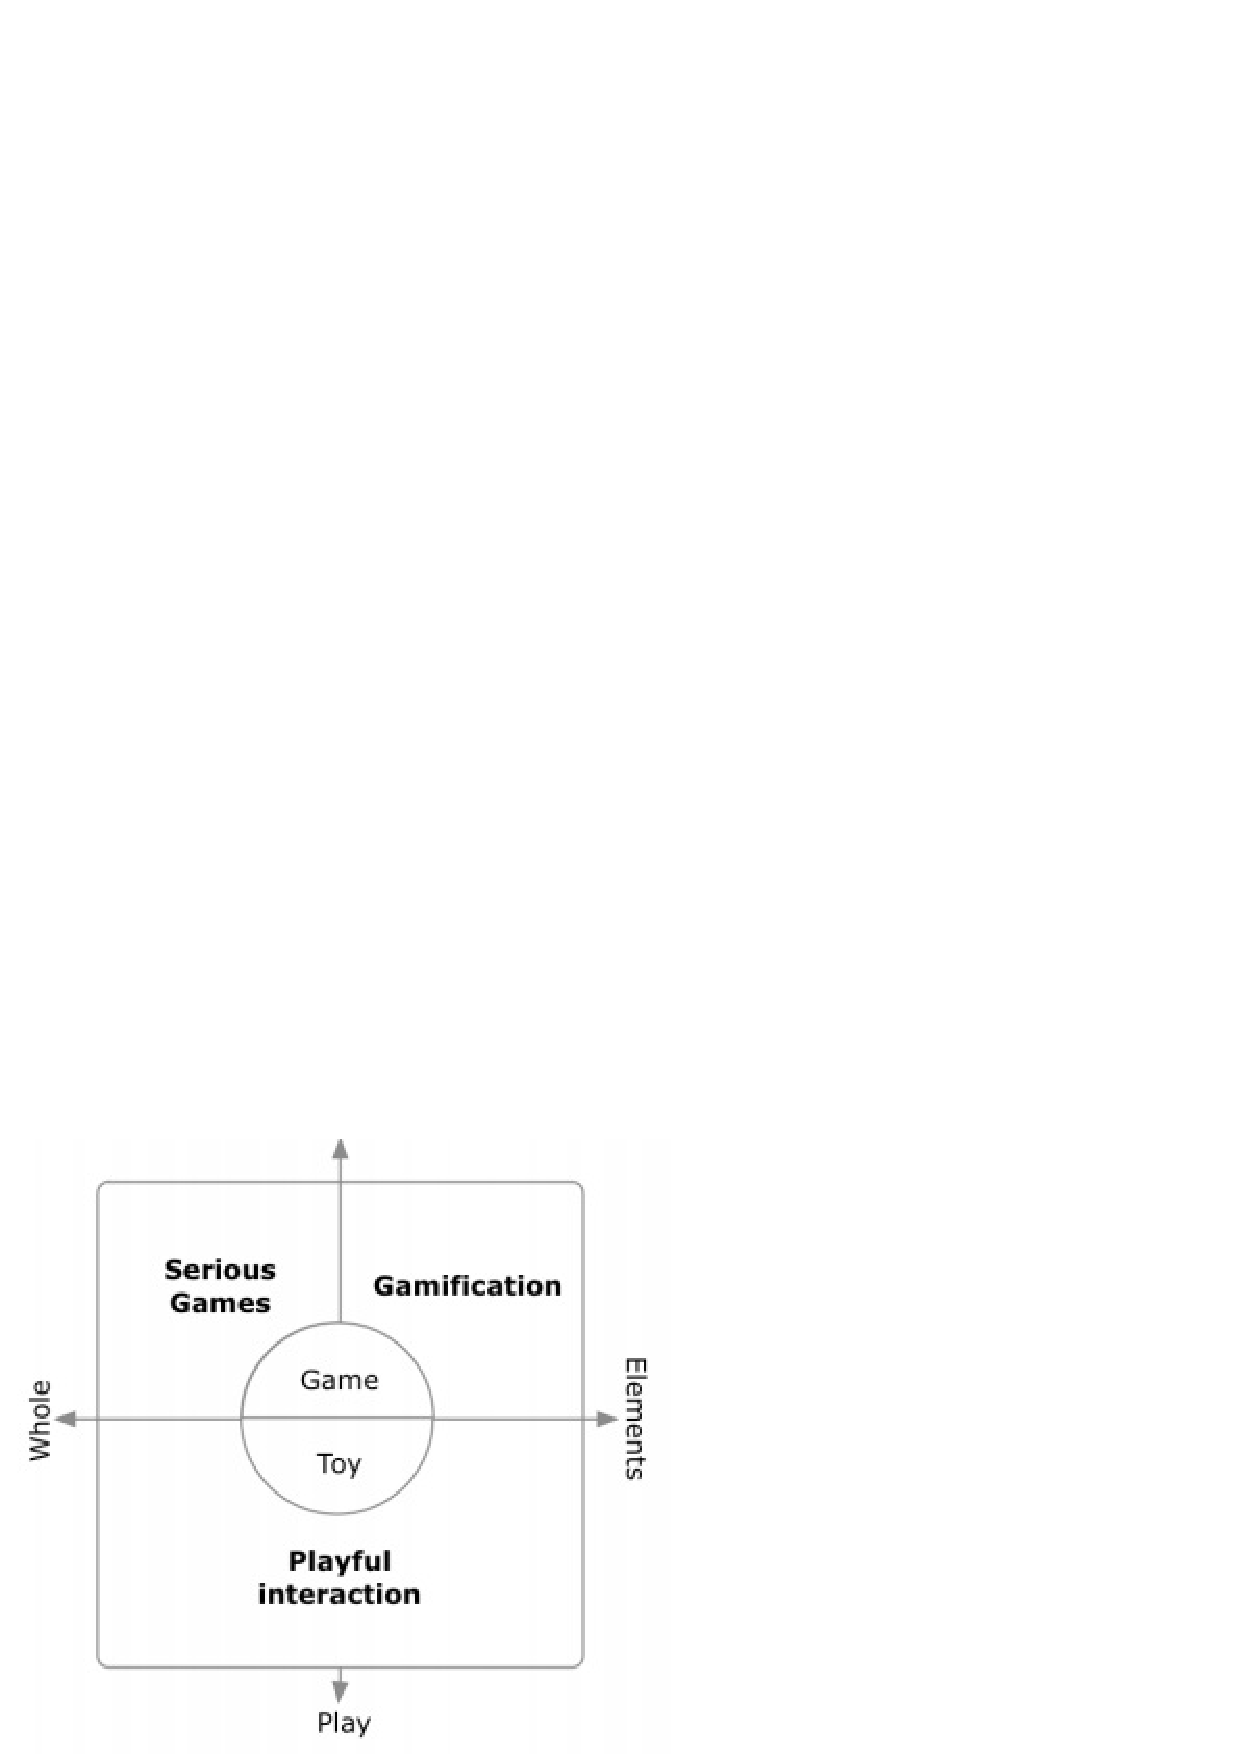
\includegraphics[scale=0.55]{defining_gamification.jpg}
		\caption{Defining Gamification (source: Deterding \cite{Deterding2011mt})}
		\label{fig:define_gamification}
\end{figure}

\section{Gamification Examples}
There are many examples of applications that effectively employ game design elements. We will only briefly examine a few here for the purpose of better understanding the gamification concept and how it is utilized across a wide range of everyday life. The following examples are selected with the hope to cover the broad range of influential gamification cases. The list here is in no way the completed list. In this quickly evolving landscape, there may well be a risk of missing some eminent ones.

\subsection{FourSquare : Check-in to Unlock}
FourSquare \cite{foursquare} is a location-based game-like service where players check-in to locations for virtual points and rewards. It is probably the most recognized forerunner of applying game mechanics to location-based networking application. By employing gamification elements such as points, badges, levels and leader boards, it engages users to revisit a location such as restaurant or pub and become a loyal customer and finally the ``mayor'' of the place. Some virtual rewards such as the ``mayors'' of Starbucks or certain badges could be converted into real products, e.g. a free coffee. Foursqure proved that simple game mechanics can affect user behavior by engaging 10 million customers with a successful business model.

\begin{figure}[htbp]
	\centering
		\includegraphics[scale=0.25]{foursquare.pdf}
		\caption{Foursquare makes modern badges popular}
		\label{fig:foursquare}
\end{figure}

\subsection{Nike+: Making Fitness Fun}
Nike+ \cite{nikeplus} is a social running game-like application that employs game mechanics to encourage runners - both casual and hardcore - to compete and improve their fitness, with the goal to solve the main problem of most fitness programs: motivation. Nike+ makes it easy for runners to upload their exercise data to its web site, and start challenging themselves and their friends. They can also get supports from their friends through the web site. The game makes running and exercise fun.

\begin{figure}[htbp]
	\centering
		\includegraphics[scale=0.2]{nikeplus.jpg}
		\caption{Nike+ makes fitness run}
		\label{fig:nikeplus}
\end{figure}

\subsection{Microsoft RibbonHero - Making You Better Your Job} 
RibbonHero \cite{ribbonhero} is a game that helps users discover new Microsoft Office features in a fun and motivating way. The goal is to have users build familiarity and expose them to the Office UI, so that they understand what kind of features are available. According to the creator of the game, Office ``has a lot of powerful features that users might not know but can be really useful''. The game gives users a chance to learn those features in a fun and engaging way, rather than reading the software manuals or watching the typically dry IT training videos. 

\begin{figure}[htbp]
	\centering
		\subfigure[Quest to earn points]{\label{fig:Ribbon1}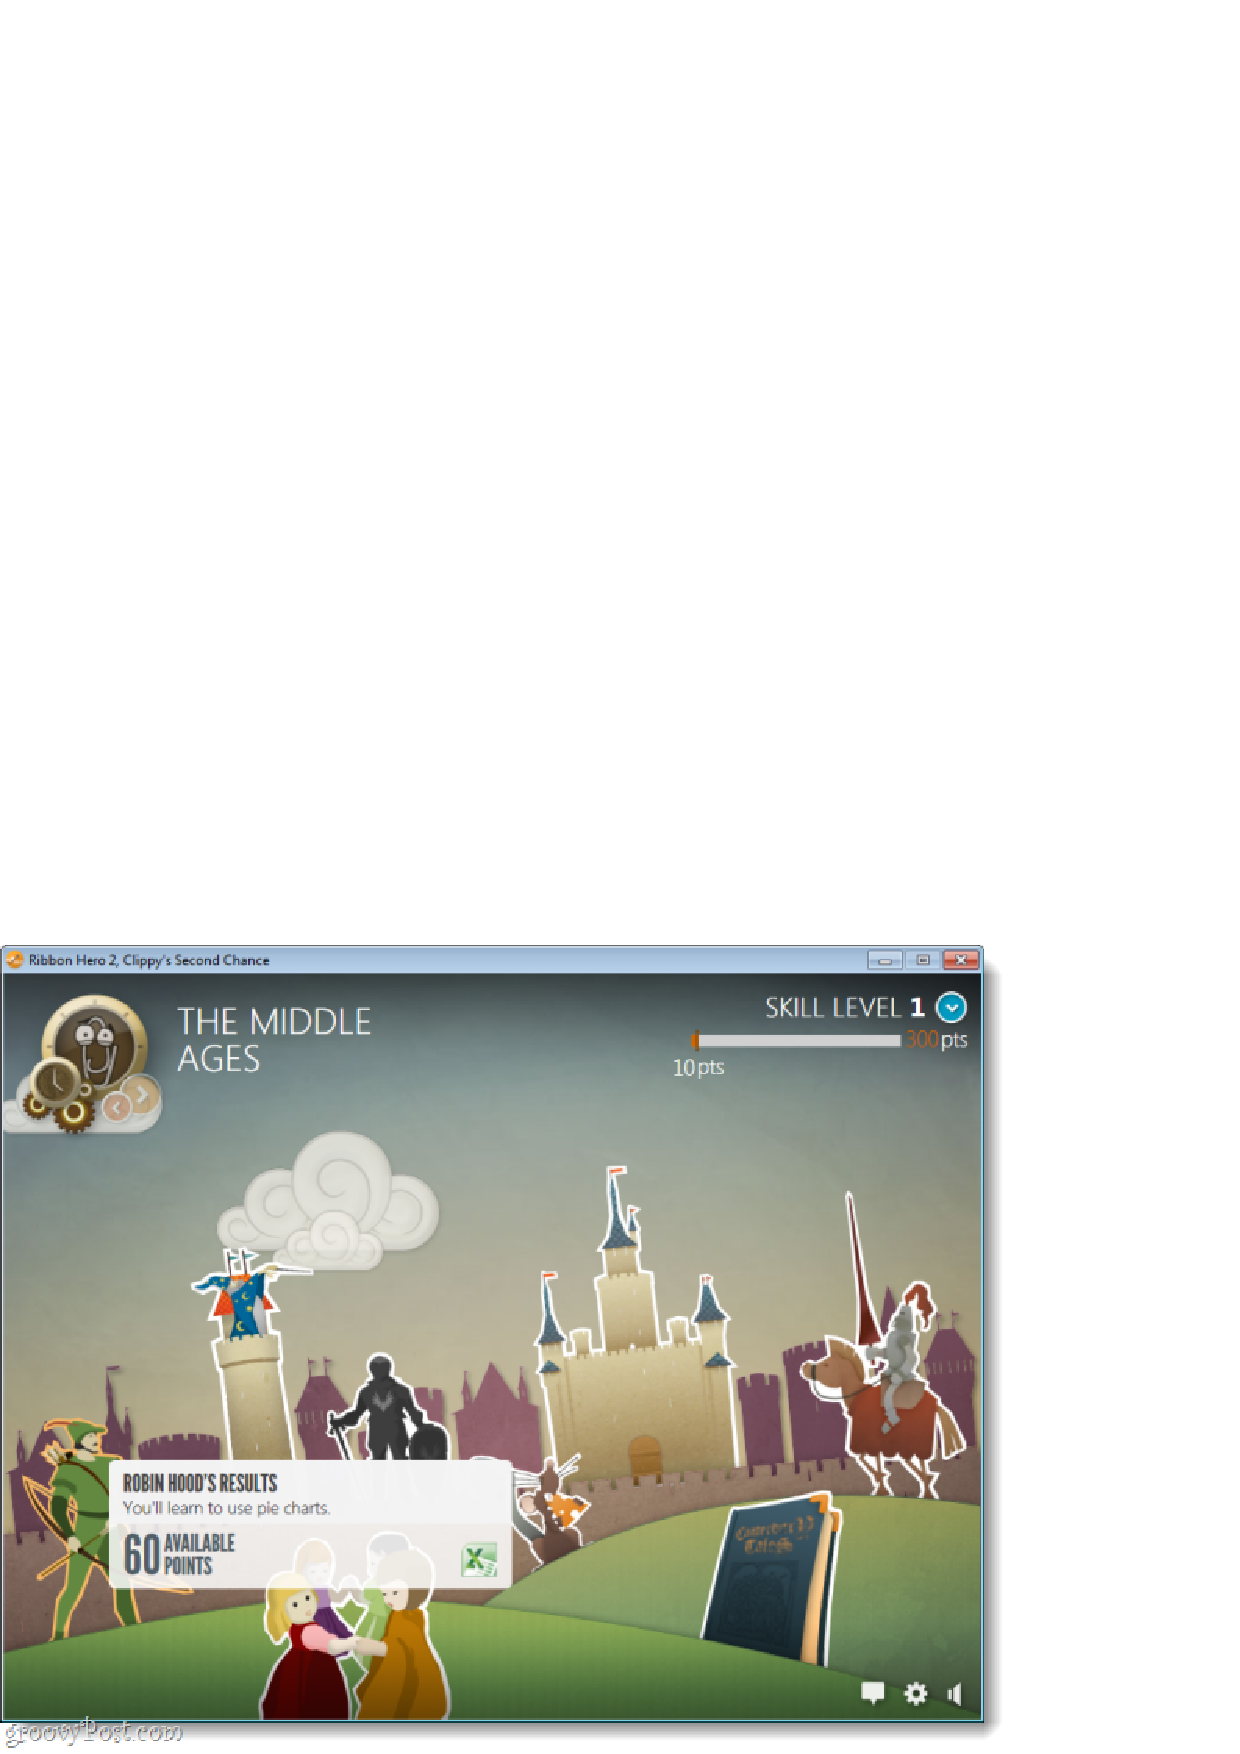
\includegraphics[height=2in]{ribbon1.png}}
		\subfigure[Competing a task]{\label{fig:Ribbon2}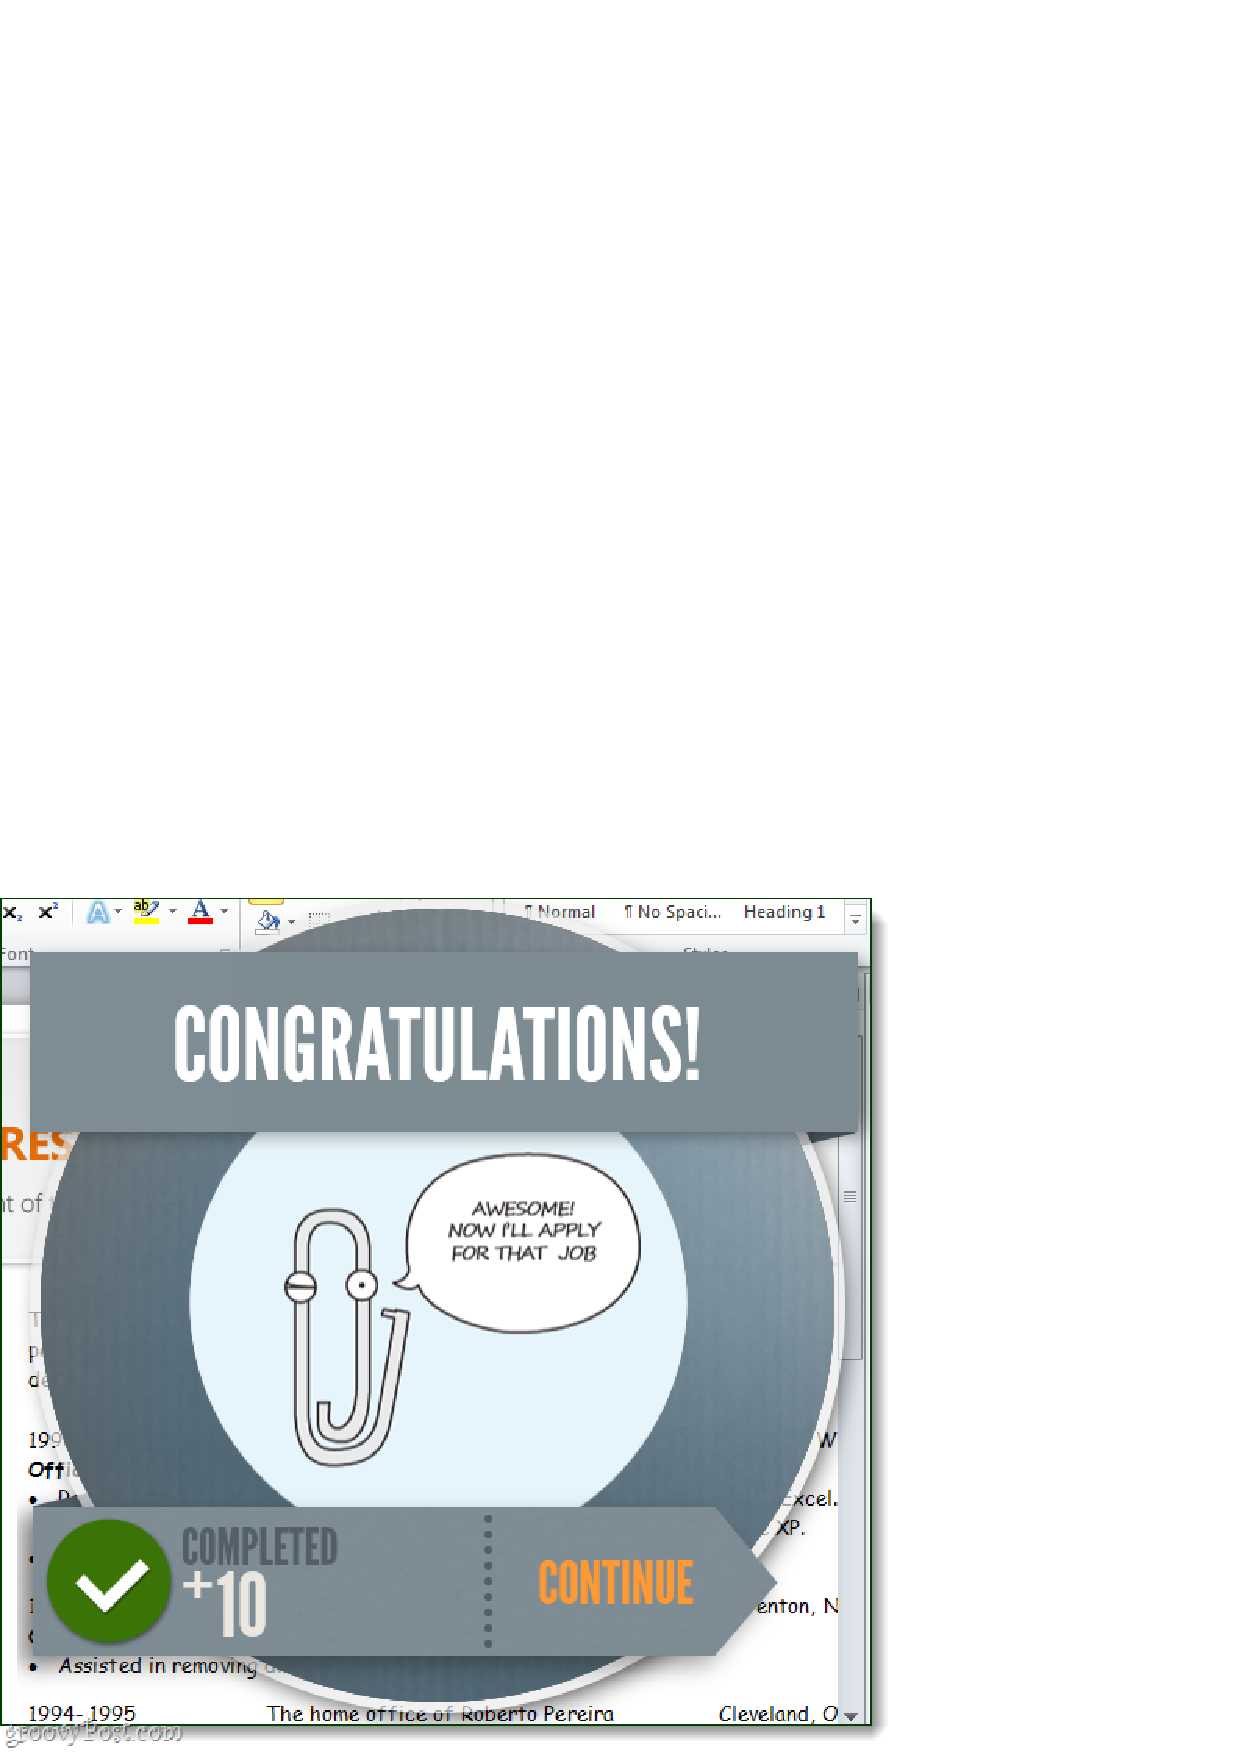
\includegraphics[height=2in]{ribbon2.png}}
		\caption{RibbonHero Helps to Learn Office}
		\label{fig:ribbon}
\end{figure}

\subsection{RecycleBank - Making the World Sustainable}
RecycleBank \cite {recyclebank} introduced a series of ``Green Challenges'' that used gaming techniques to motivate participants to learn about green living and to take small green actions to live more sustainable lives. According to their report \cite {gamingforgood}, 49,000 individuals participated in the ``Green Your Home Challenges''. Partnered with Google Analytics and ROI research, they found that:
\begin{itemize}
	\item Gamification can increase awareness of positive environmental actions. 97\% of participants surveyed said the game increase their knowledge of environment.
	\item Games can drive individuals to take positive social and environmental actions. Most participants surveyed indicated they are very or extremely likely to take green actions as a result of participating in the challenge. 
	\item Games are an effective and appealing educational tool. 86\% participants agreed online games and contest can be a good way to inform and educate them personally. 
\end{itemize}

\begin{figure}[htbp]
	\centering
		\subfigure[Green Your Home Challenge]{\label{fig:RecycleBank1}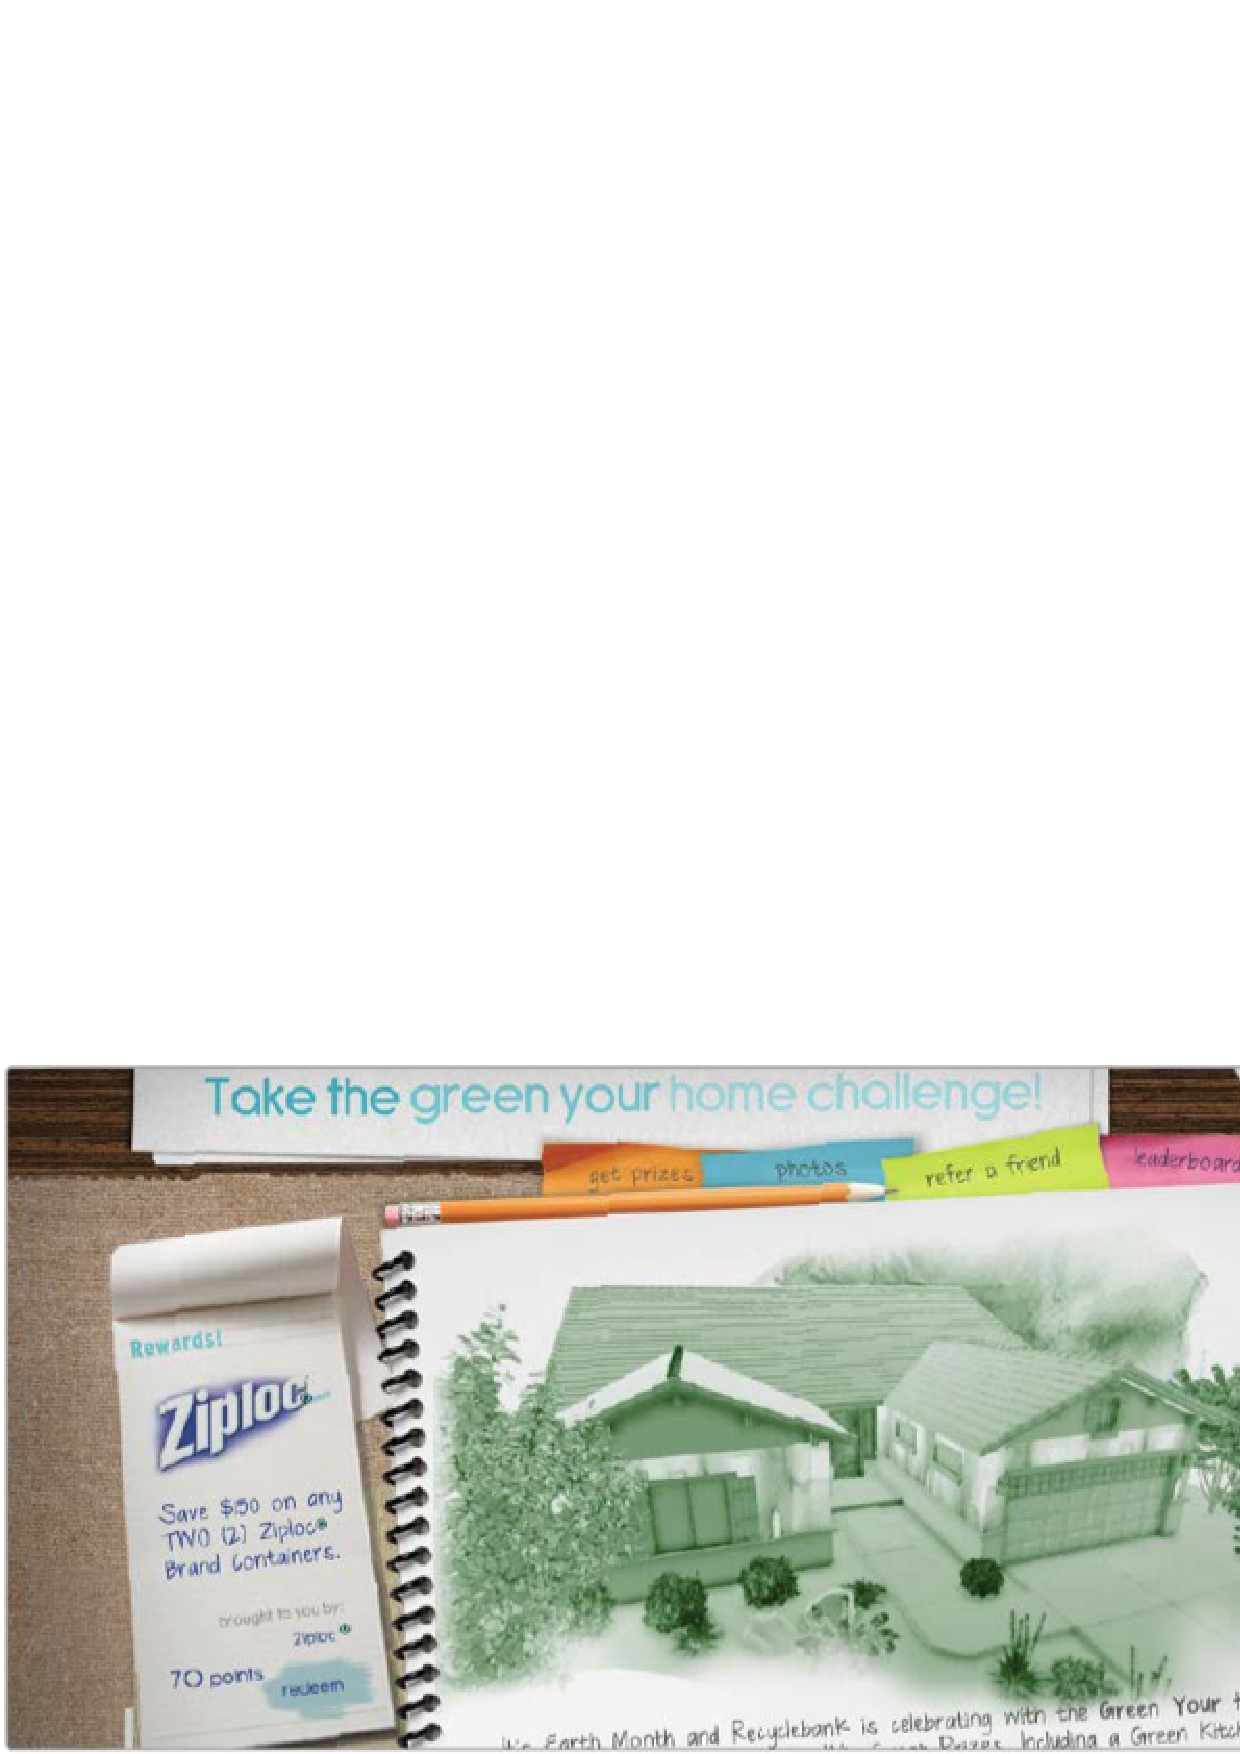
\includegraphics[scale=0.3]{recyclebank1.png}}
		\subfigure[Game Change Behavior]{\label{fig:RecylceBank2}
\includegraphics[scale=0.65]{recyclebank2.png}}
		\caption{RecycleBank - Gaming for Good}
		\label{fig:recyclebank}
\end{figure}	

\section{Why Games and Now}

Gamification is not about games. In fact, the subjects of gamification deal with everything else but games. However, to understand the research in gamification, we have to look at the studies of games. The games already prove to be an effective engaging media and ubiquitous as every day life. "Video game is everywhere" is the critical thesis of many gamification advocates. 

Why game? Results of a study published in the May 1998 issue of Nature \cite {koepp1998evidence} demonstrated that video game players experienced regular releases of dopamine during game play. Dopamine is a
neurotransmitter that signals pleasure rewards for food, sex and addictive drugs, such as cocaine. This and subsequent studies have proven that playing games stimulates pleasure centers in the brain. People are hard-wired to enjoy games.

Carnegie Mellon University professor and game designer Jesse Schell, who ignited the first wave of interest in gamification with a keynote address at the 2010 Design Innovate Communicate Entertain (D.I.C.E.) Summit, mentioned that he was surprised so many people took interest in his presentation now. He had talked about the phenomenon for years with little response. Back in 2008, Gabe Zichermann coined the term "funware", which is the use of game mechanics to encourage desired user actions and generate customer loyalty \cite {WikipediaFunware}. Although it has the similar concept as gamification, the term ``funware'' did not gain enough traction then.

Why Now? According to Schell, ``We're moving from a time when life was all about survival to a time when it was about efficiency into a new era where design is largely about what's pleasurable''. Online games have entered the mainstream and become the new revolution of culture shift, helped by platforms such as smart phones, tablets and Facebook. Gamification is a way to arrive at a ``fundamental understanding of what it is that's pleasurable to people'' from many aspects of life. 

Stanford professor Byron Reeves describes that a ``Game Tsunami'' is happening now in his book ``Total Engagement'' \cite{reeves2009total}. According to him, ``Games Are Big'' in three ways: 

1. Big Bucks. Game industry is already a \$10 billion market, one of the largest existing entertainment categories.  Besides the traditional console and software sales, the current model of subscription fees, virtual goods sales and in-game purchase also account for the huge revenue for the game industry.

2. Big People. The stereotype about the majority gamers are unemployed youth is easily proved wrong. One research reveals that across all computer games, the average age of gamers is 35, and 26\% of players are over 50, an increase from 9\% in 1999. Another research shows the mean household income of players in one popular MMO (Multi-Player Online game) was about \$85,000, and almost two-thirds of the players have some college education.

3. Big Time. ``One sizable cohort of players who are thirty-something, most with a full-time job and many with a family, play MMOs over 25 hours per week, compared with 7 hours  a week for all video games''.

On the similar landscape, researcher and game designer Jane McGonigal advocates playing game is the solution to the "Broken Reality" \cite{mcgonigal2011reality}. She notes that currently more than 3 billion hours a week is spent in playing video game by our society, for good reasons. She says that the average gamer plays 10,000 hours of games by age 21. That�s about the same number of hours that students spent in high school and middle school. There are 500 million gamers today, playing on all sorts of platforms from the iPhone to the game consoles. Instead of the common conception that gaming is a waste of time, she argues that ``playing games is the single most productive thing we can do with our time''.

In the British Museum's department of Greek and Roman antiquities, there is an exhibition section about ancient games. The description of the exhibition states that ``We know very little about how most ancient games were played. Their rules were probably too familiar for people to take the trouble of writing them down''.  A favorite subject of Greek vase-painters was Ajax and Achilles playing a kind of board game called backgammon as illustrated in Figure 2.7. It is noteworthy that both Ajax and Achilles have the full armor on while playing the game. According to Arthur A. Krentz, Plato's ``Republic'' described the connection between play and education of both adult and children. He points out that, the term ``paideia" (in Greek, means education/culture), ``paidia" (means play/game/pastime/sport), and ``paides" (means children), have the same root. The three terms often show up in the same context. ``The central aim of pedagogy (paidagogia) is to encourage learning as a form of play (paidia), which is the most persuasive and effective approach to learning" \cite{krentz1998play}.

Another game artifact exhibited in the museum is a set of label-shaped ivories, inscribed on one side with words and on the other with numbers. The series of numbers run from 1 to 25. The higher numbers have inscriptions of complimentary words, such as FELIX ("lucky") and BENIGNE ("kindly") \cite{walters1929guide}. The pieces may have been used in the Roman game called "the game of soldiers". One can relate the inscribed ivory pieces to the badges in modern games.

Yet another important game antique in the museum is the Royal Game of Ur, dated from the First Dynasty of Ur, before 2600BC. It is one of the most popular games of the ancient world, and probably the oldest set of board game equipment ever found. The beauty of the equipment is still amazed by the audience today.  Wikipedia notes that the game of Ur is still played in current day Iraq. \cite {wikipediaUr}.

\begin{figure}[htbp]
	\centering
		\subfigure[Ajax and Achilles Playing]{\label{fig:roman-game-vase}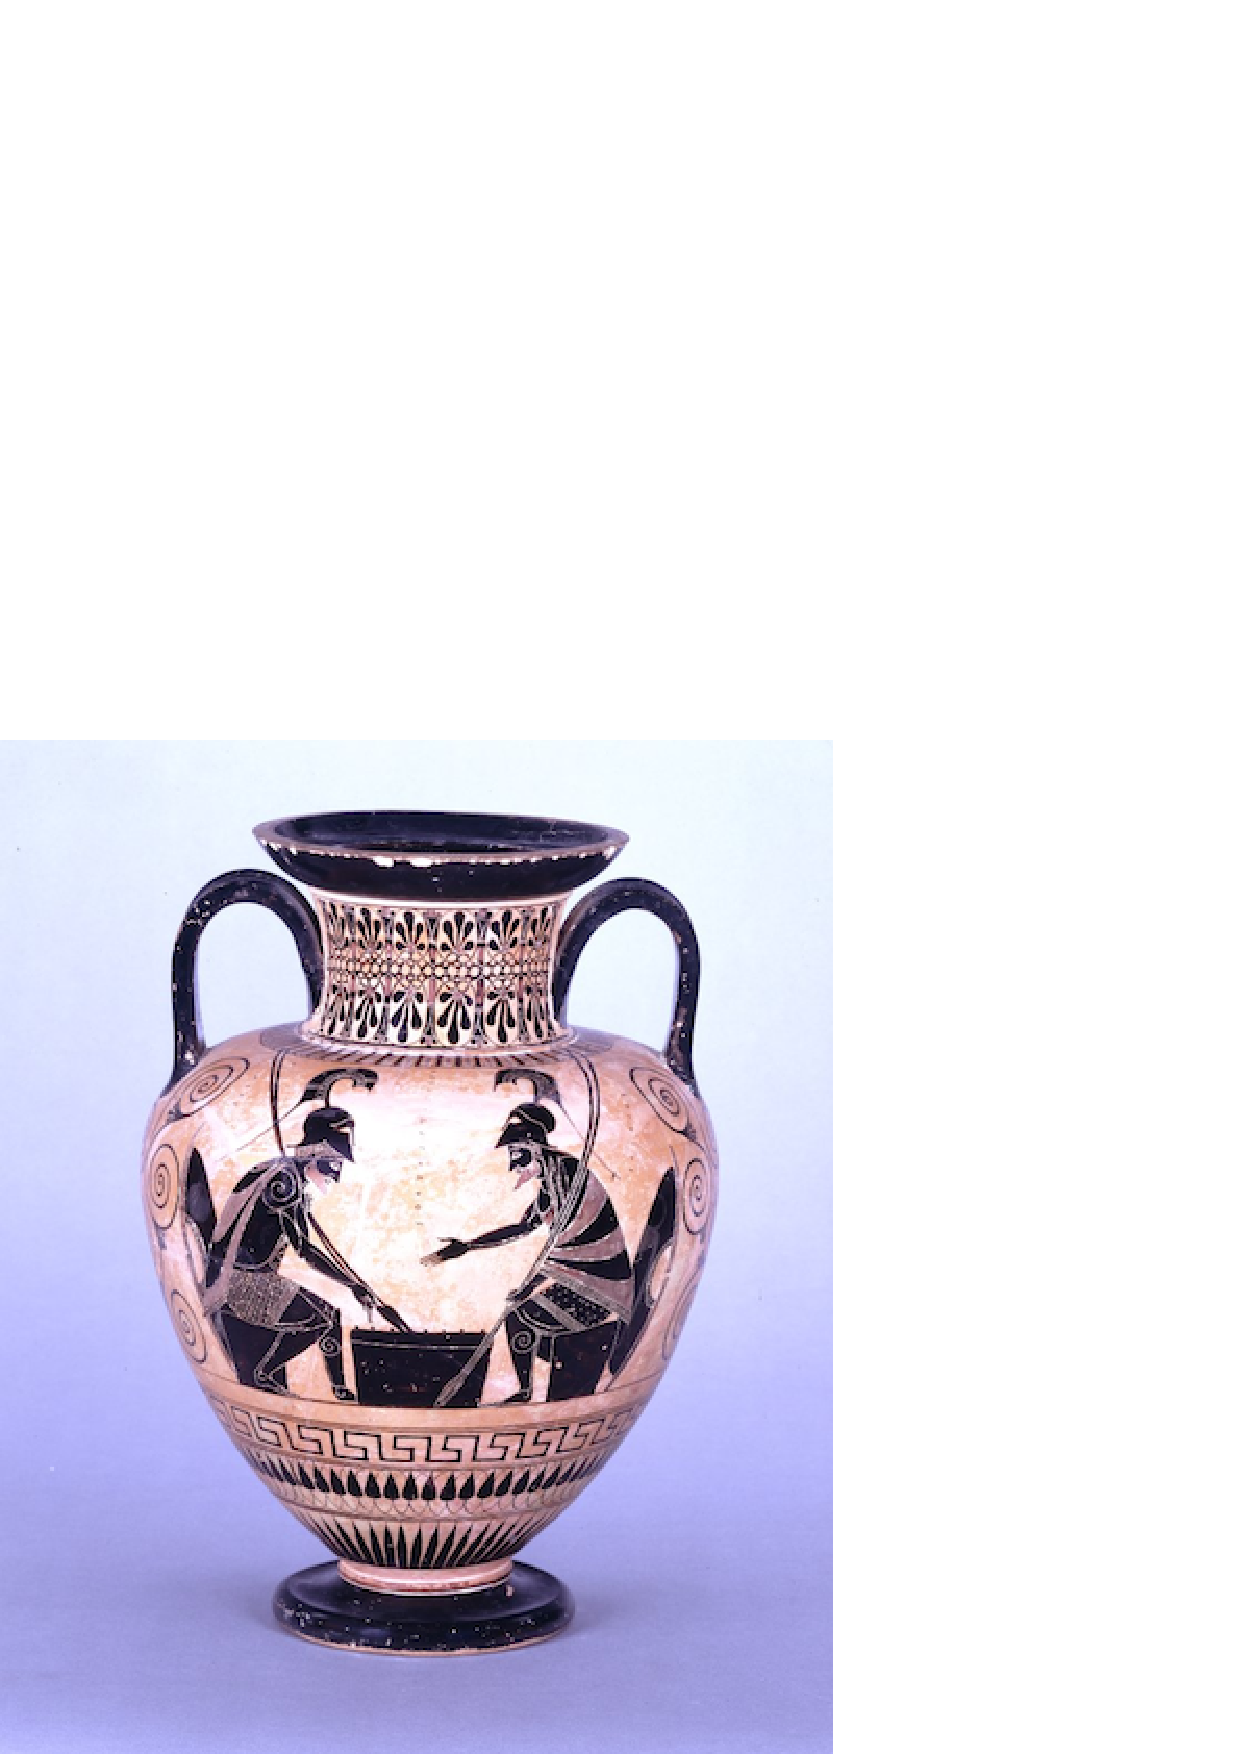
\includegraphics[height=2in]{roman-game-vase.png}}
		\subfigure[Ancient Game Badges]{\label{fig:roman-game}\includegraphics[height=2in]{roman-game.png}}
		\subfigure[The Royal Game of Ur]{\label{fig:boardgame-ur}\includegraphics[height=2in]{boardgame-ur.jpg}}
		\caption{The Beauty of Ancient Board Games in British Museum}
		\label{fig:ancient-board-games}
\end{figure}

World of Warcraft (WoW) is a massively multiplayer online role-playing game (MMORPG) with 11.1 million subscribers, currently the world's most popular MMORPG.  More than 50 billion hours have been spent in playing the game since the start of this game in 2004. The players created 250,000 articles in the WoW-Wiki, the second largest wiki behind Wikipedia. On average each WoW-player spends from 17 to 21 hours per week playing WoW.

Nick Yee describes 5 motivation factors why people play MMORPGs \cite {yee2002facets}:  (1) Relationship: This factor measures the desire to develop meaningful relationships with other players in the game - usually in the form of a supportive friendship. (2) Immersion: This factor measures the desire to become immersed in a make-believe construct. Players who score high on this factor enjoy being immersed in a fantasy world they can wander and explore. (3) Grief: This factor measures the desire to objectify and use other players for one's own gains. Their means may be both outward or subtle by killing or deceiving. (4) Achievement: This factor measures the desire to become powerful within the construct of a game. Players who score high on this factor try to reach the goals as defined by the game. (5) Leadership: This factor measures the gregariousness and assertiveness of the player. Players who score high on this factor prefer to group rather than solo. 

Yee also noted that most of the activities offered by a MMORPG are already present in single player games. What makes a difference is apparently the shared experience, the collaborative nature of most activities and, most importantly, the reward of being socialized into a community of gamers and acquiring a reputation within it. ``It�s the people that are addictive, not the game'' \cite {yee2002understanding}. 

He claimed that ``WoW truly is a virtual Skinner box'', smoothly increasing reward and difficulty and reinforcing player commitment along the way \cite {yee2001vsb}. Players are always on the edge of opening up new abilities, of discovering new content. 

Based on longitudinal data collected directly from playing the game, Ducheneaut et al. described that many of WoW�s subscribers play alone with a different kind of social factor, ``audience", a sense of social presence \cite {ducheneaut2006alone}. It is different than the quest grouping that providing direct support and camaraderie. There are three appeals in being "alone together" in multiplayer games: (a) interacting with an audience: MMORPGs are in essence reputation games - an avatar wearing powerful items, for instance, is essential to the construction of a player�s identity (b) being surrounded by others. (c) laughing at and with others.
	
\section{Why Gamification}

In her popular and inspiring TED talk ``Gaming can make a better world" \cite {mcgonigal2010ted} and in her book ``Reality is Broken" \cite {mcgonigal2011reality}, researcher and game designer Jane McGonigal illustrated why good games make us better, and how they can help us change the world. She said "Reality is broken", and game is the fix. Games are nothing more than ``unnecessary obstacles'' that we volunteer to tackle. Why are we spending so much time on unnecessary obstacles? McGonigal says it has a lot to do with ``eustress'' or positive stress. Based on the findings of positive psychology, She argues that the blissful productivity comes from the flourishing feeling, such as positive emotion, relationships, meaning and accomplishments.

Another instrumental work came from Byron Reeves's book ``Total Engagement" \cite {reeves2009total}.
He argues that games, especially MMO type games, can change the ways people work and businesses compete. He illustrates ten ingredients of great games and how to use them to design a better productive work place:
(1) Self-representation with avatars. (2) Three-dimensional virtual environments. (3) Narrative context. (4) Feedback. (5) Reputations, ranks, and levels. (6) Marketplaces and economies. (7) Rules that are explicit and enforced. (8) Teams. (9) Communication system that can be reconfigured by participants. (10)Time pressure.  

In his book ``Game Based Marketing" \cite {zichermann2010game}, Gabe Zichermann stated that ``FunWare" is about taking the lessons learned from the game industry and bake them into any kind of life experience. Marketing has always been about a certain degree of persuasion and motivation, and a degree of manipulation. Games do that most effectively. ``Game mechanics and the psychological conditions are powerful tools that marketers can use, and they are a lot cheaper ... than cash in the long run". ``Games are the only force in the known universe that can get people to take actions against their self-interest, in a predictable way, without using force". This resonates the volunteering attribute of game play in McGonigal's book.

\section{Science behind Gamification: Motivation and Behavior Change}
Researchers from game industries and academia, have studied the psychology of motivation that makes games so engaging. 

\subsection{Flow}
Psychology professor Mihaly Czikszentmihalyi introduced a specific kind of happiness that he named ``flow" \cite{csikszentmihalyi1991flow}, which is considered as one of the fundamental reasons that people play games \cite{murphygames}. Flow is a state of absorption, characterized by intense concentration, loss of self-awareness, a feeling of being perfectly challenged (neither bored nor overwhelmed) and a sense that time is flying. 

Csikszentmihalyi describes that there are seven core components of flow, as  summarized in Table 2.1 \cite{csikszentmihalyi1991flow}. These components can be broken into two categories: conditions and characteristics. Conditions must be achieved before flow can be reached. Characteristics occur while a person is in flow, even though they may be unaware of it.

\begin{table}[htbp]
  \centering
    \caption{Flow Condition and Characteristics (source: Czikszentmihalyi \cite{csikszentmihalyi1991flow})}
    \begin{tabular}{ | l | p {10cm} |}
    \hline
    Conditions of Flow & Explanation \\ \hline
    Clear tasks & Person understands what they must complete  \\ \hline
    Feedback & Person receives clear and immediate feedback showing what succeeds and what fails \\ \hline
    Concentration/focus & Person is not distracted and can fully attend to the task \\ \hline
    An attainable, balanced goal & Goal is challenging and within their abilities to complete \\ \hline
    Characteristics of Flow & Explanation \\ \hline
    Control & Person believes their actions have direct impact on tasks and that they can control the outcome \\   \hline
    Diminished awareness of self & Complete focus on the task leaves little room for feeling self-conscious or doubt. Often described as becoming a part of the activity. \\ \hline
    Altered sense of time & Perception of time is distorted. Seconds can feel like minutes, minutes like hours. Yet, time also passes by quickly, unnoticed. \\ \hline
    \end{tabular}
\end{table}

In order to achieve the flow, the right conditions above must exist. The last and the most important condition is a balanced goal that is challenging yet achievable within the individual's ability. A task that is not challenging or  requires excessive time to complete becomes boring and players lose interest; A task that is too hard causes frustration and anxiety and again players lose interest. With a person's skills improve over time, the challenge needs to increase along with the improving skills. This balance is referred to as the flow channel as shown in figure 2.7.

\begin{figure}[htbp]
	\centering
		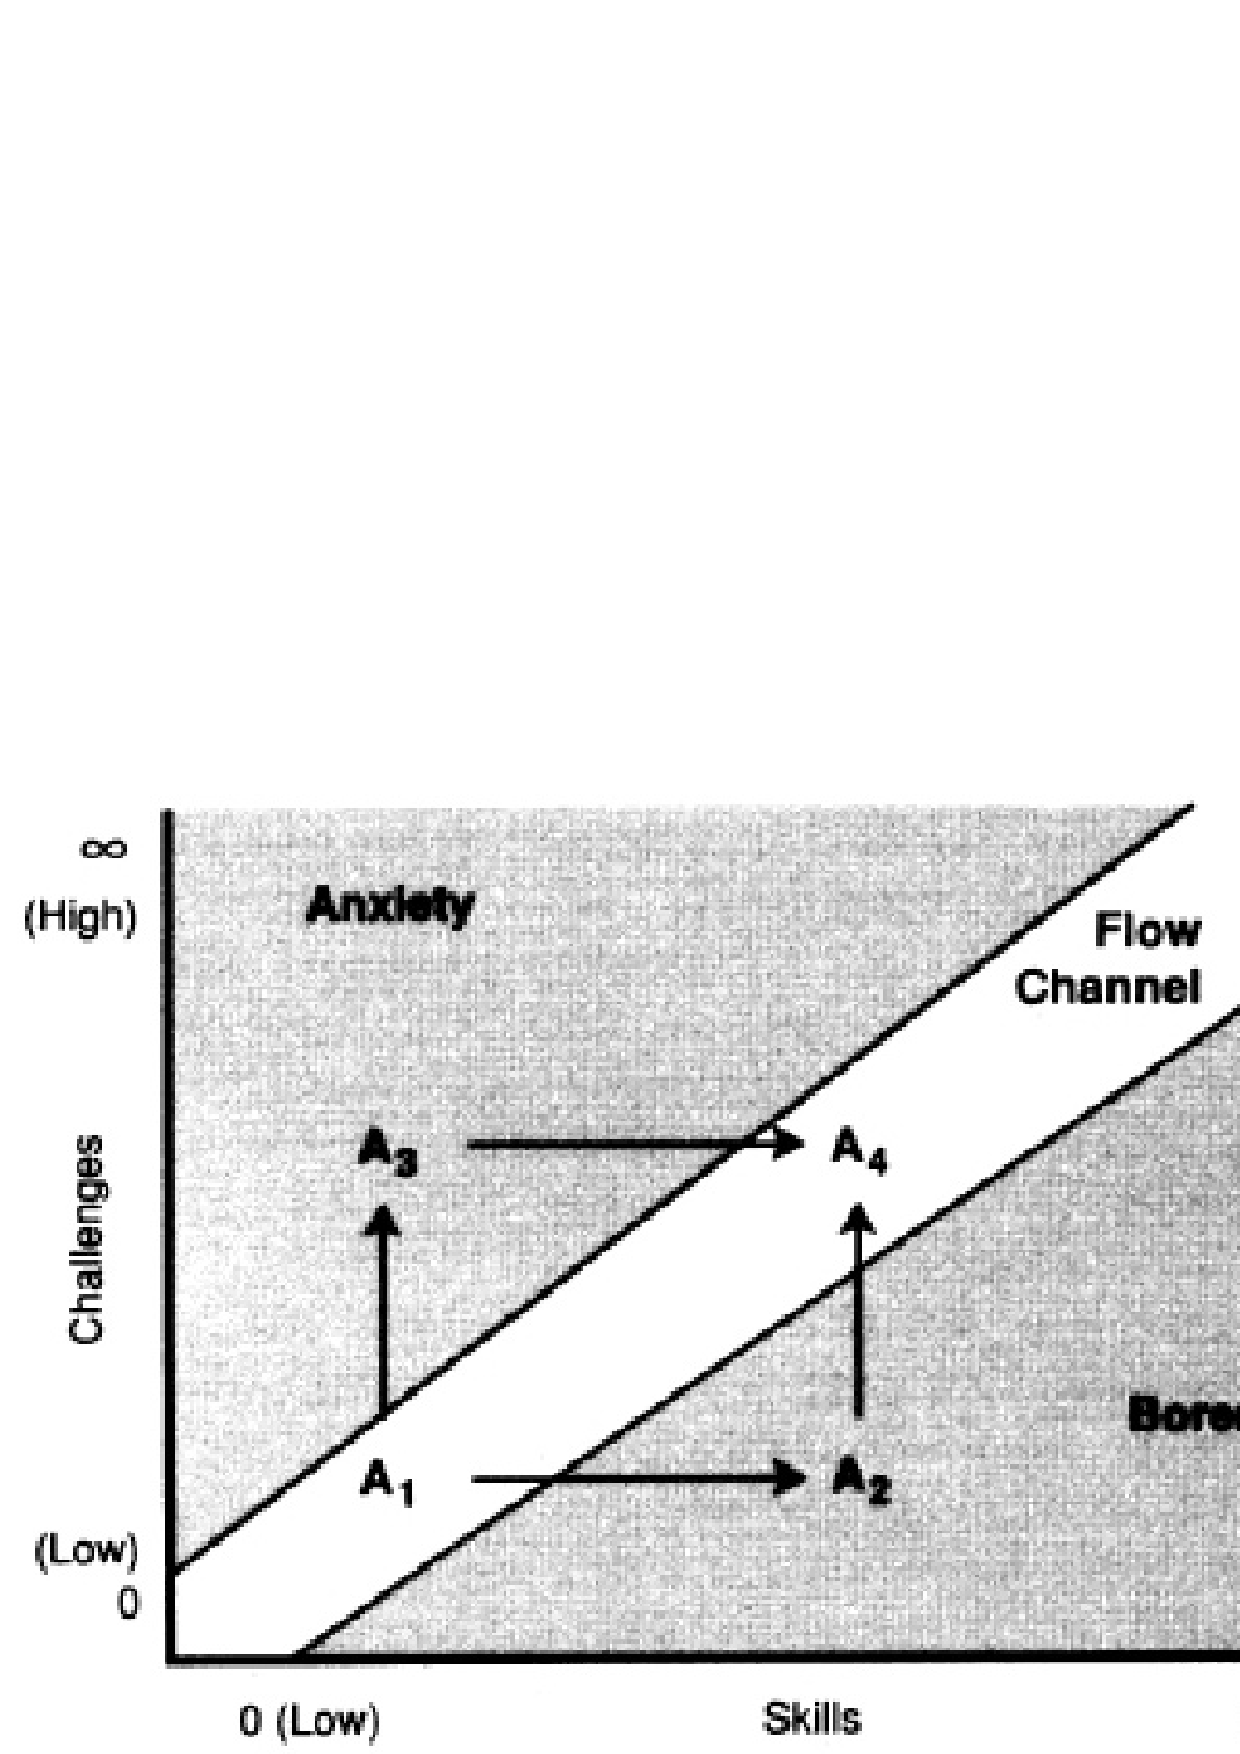
\includegraphics[scale=0.45]{flow.jpg}
		\caption{The state of flow is achieved between anxiety and boredom (source: Czikszentmihalyi \cite{csikszentmihalyi1991flow})}
		\label{fig:state_of_flow}
\end{figure}

\subsection{Player Type}
In order to understand why people play games, Richard Bartle identified four player personality types by studying players of the Multi-User Dungeon (MUD) game in 1960s \cite {bartle1996hearts}. The four types are based on the 2 underlying axes: 

1. Achievers: driven by in-game goals, usually some form of points gathering - whether experience points, levels, or money.

2. Explorers:  driven to find out as much as they can about the virtual construct - including mapping its geography and understanding the game mechanics.

3. Socializers: use the virtual construct to converse and role-play with their fellow gamers.

4. Killers: use the virtual construct to cause distress on other players, and gain satisfaction from inflicting anxiety and pain on others.

Bartle's player type model has been the basic for understanding the player motivation. Dan Dixon presented the limitation and misuse of Bartle's model in general games and gamification contexts \cite{DixonPlayerType}. Amy Jo Kim applied the model in her gamification approach by overlaying social actions from the game on top of the player types \cite {Kim2010}, as shown in Figure 2.8.

\begin{figure}[htbp]
	\centering
		\subfigure[Bartle's Player Types (1996)]{\label{fig:player-types}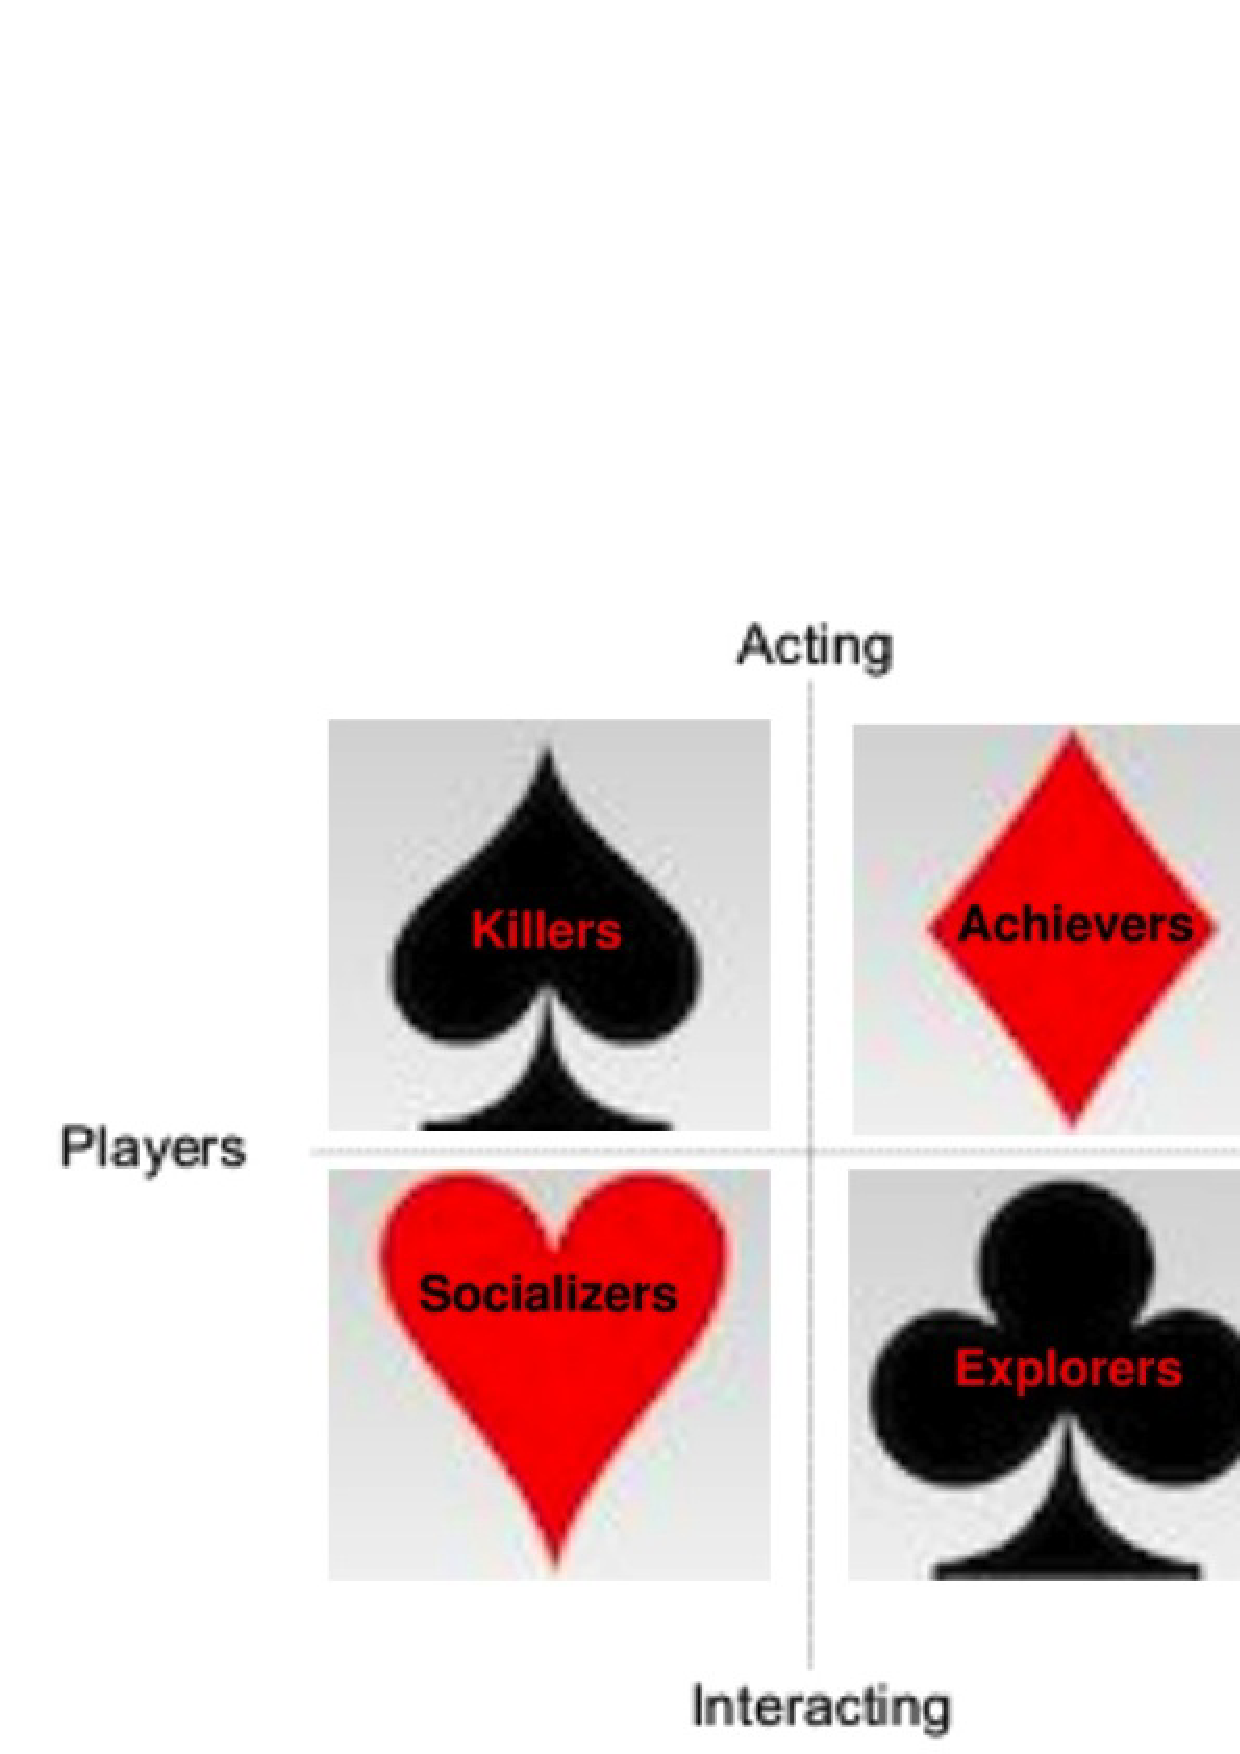
\includegraphics[height=2.0in]{bartle-player-types.jpg}}
		\subfigure[Kim's Social Actions (2010)]{\label{fig:social-action}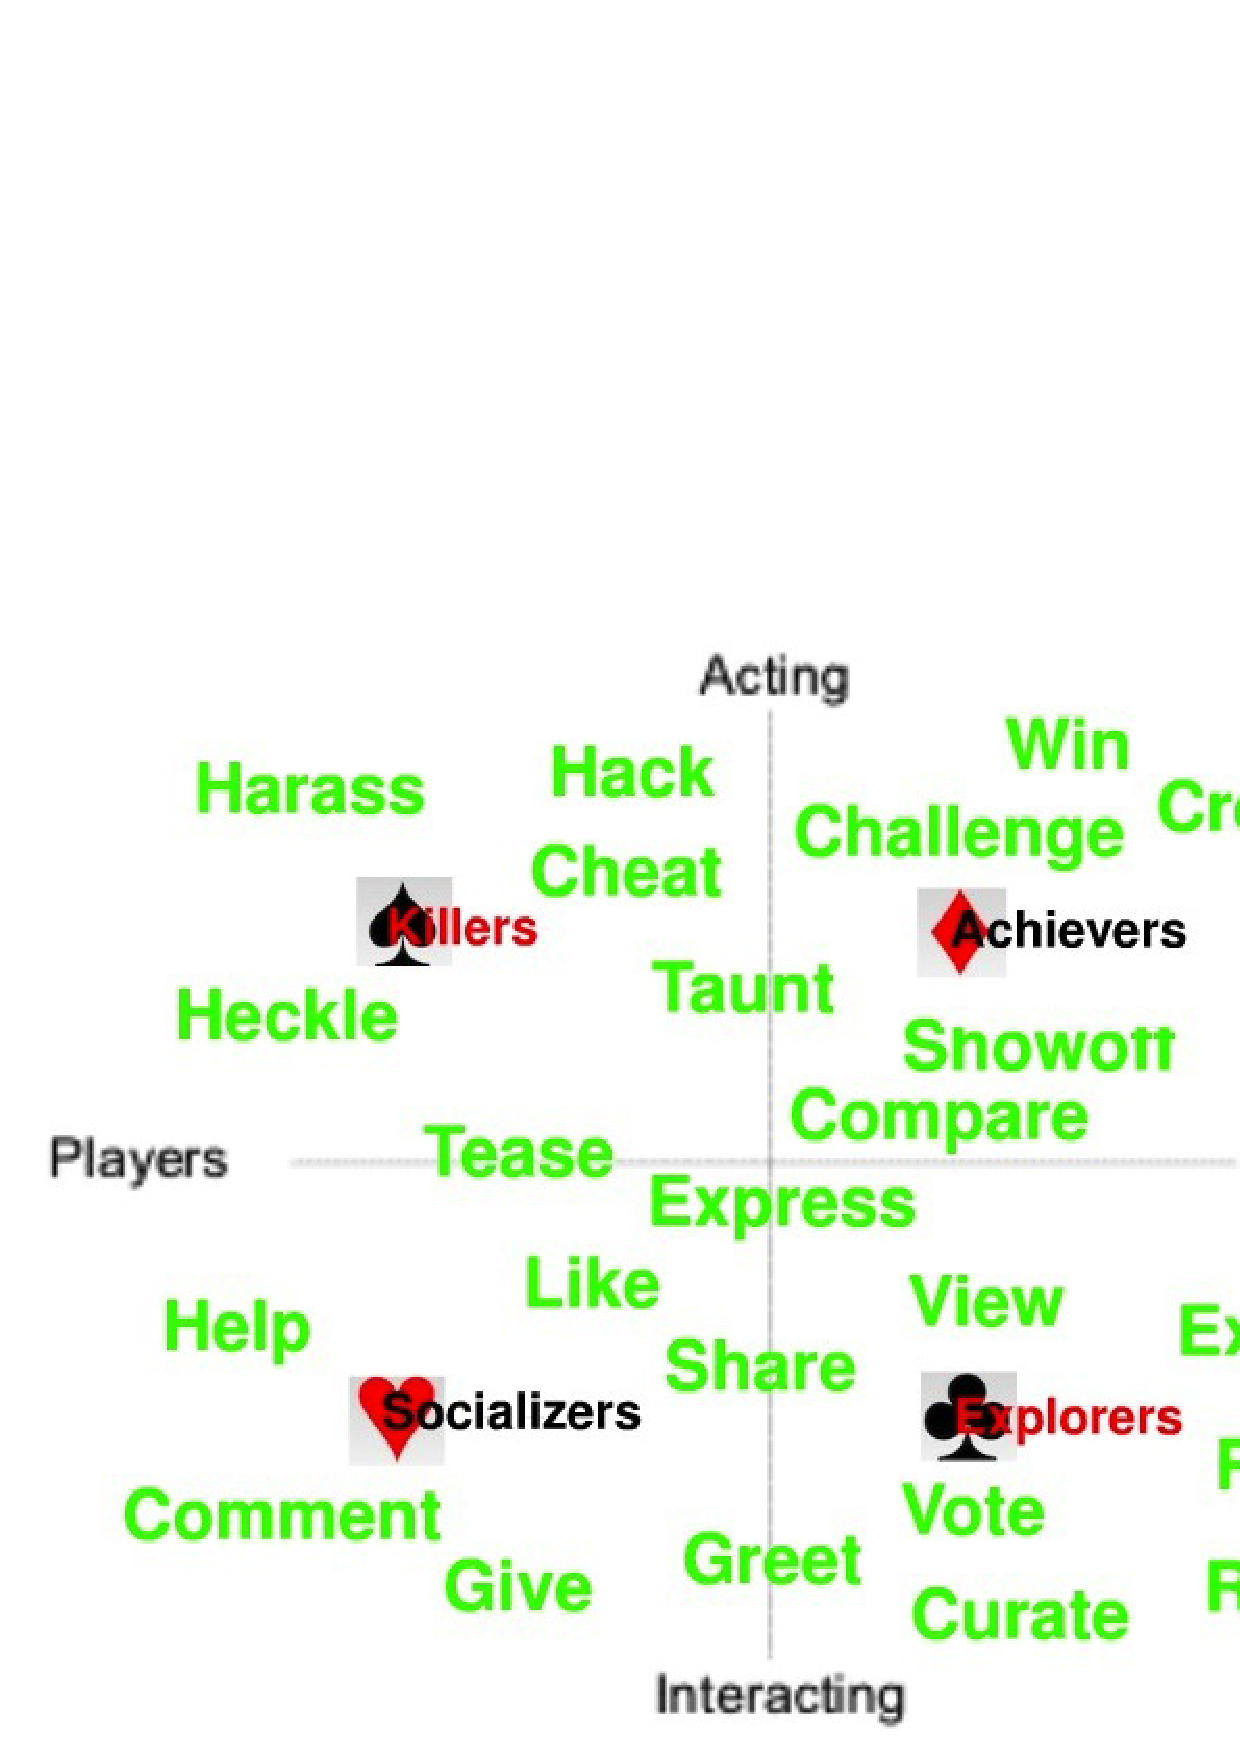
\includegraphics[height=2.0in]{kim-player-types.jpg}}
		\caption{Player Types}
		\label{fig:play-types}
\end{figure}

\subsection{Fogg Behavior Model}
Stanford University researcher BJ Fogg introduces the Fogg Behavior Model (FBM) to explain what causes behavior change \cite {fogg_2003}. The model shows that three elements must converge at the same moment for a behavior to occur:

1. Motivation: the person wants desperately to perform the behavior (i.e. he is highly motivated)

2. Ability: the person can easily carry out the behavior (i.e. he considers the behavior very simple)

3. Trigger: the person is triggered to do the behavior (i.e. he is cued, reminded, asked, called to action, etc.)

\begin{figure}[htbp]
	\centering
		\includegraphics[scale=0.55]{fogg_behavior_model.jpg}
		\caption{Fogg Behavior Model (source: Lithium \cite{Wu2011})}
		\label{fig:behavior_model}
\end{figure}

Michael Wu uses FBM to analyze why and how gamification is able to drive actions \cite {Wu2011}. ``Game mechanics and game dynamics are able to positively influence human behavior because they are designed to drive the players above the activation threshold, and then trigger them into specific actions''. Wu suggests that gamification is an iterative process and works best when all three of motivation, ability, and trigger converge.

Another Stanford Researcher Kaptein developed a technique he called ``Persuasion Profiling'' to build a profile of which psychological triggers work best for a given person, and uses these triggers to drive new behaviors in the future \cite {kaptein2011adaptive}.  

\section{Gamification Debates and Criticism}
There are many debates and criticism over whether gamification itself is inherently good or bad. 

After his inspiring talk in DICE 2010, Jesse Schell discussed with Bryan Reynolds (Zynga chief designer) about ``Gamification vs. Gameplay" in DICE 2011 \cite {scimeca2011}. They are arguing in a very basic level of the definition of gamification. Brian considered ``Gamification is where you use game elements to try to get people to do stuff they don't want to do", while Schell responded that ``It's a problem solving situation that you enter into because you want to". Reynolds argued ``Everyone who has tried to use game mechanics to improve their marketing has only managed the most basic concepts''. Schell responded that this was the developers', not the concept�s fault.

In a debate-style session of GDC 2011, ``The Great Gamification Debate", panelists, divided by two sides, argued the merits of bringing gameplay mechanics to just about everything \cite {magrino2011}. Although they mostly agreed that definition of gamification was summed up best by Jesse Schell, ``gamification is taking things that aren't games and trying to make them feel more like games", there are a lot different opinions between the two sides. While the pro-gamification side believed the gamification is the cultural shift in every day life, the other side considered that the purpose of gamification is to cash in on the current popularity of games. While the anti-gamification side reduced the idea to merely behavioral conditioning or a kind of Skinner box for users, the pro side maintained that users should at least find a reward of values.

Designer Umair Haque argued that most gamification is about zero sum games, or artificial scarcity \cite {haque2010}. For example, many ``gamified" sites simply offer a fixed number of badges, or other trinkets.for someone to win, someone else got to lose. Designer Stephen Anderson also claimed that \cite {anderson2011}:
(a) gamification mistakes extrinsic rewards (rather than intrinsic motivation) for the power of games and hence offers only feedback, not goals \& rules,
(b) a long-term successful product or service that�s not pure entertainment most go beyond delight/entertainment and be first \& foremost useful.

\begin{figure}[htbp]
	\centering
		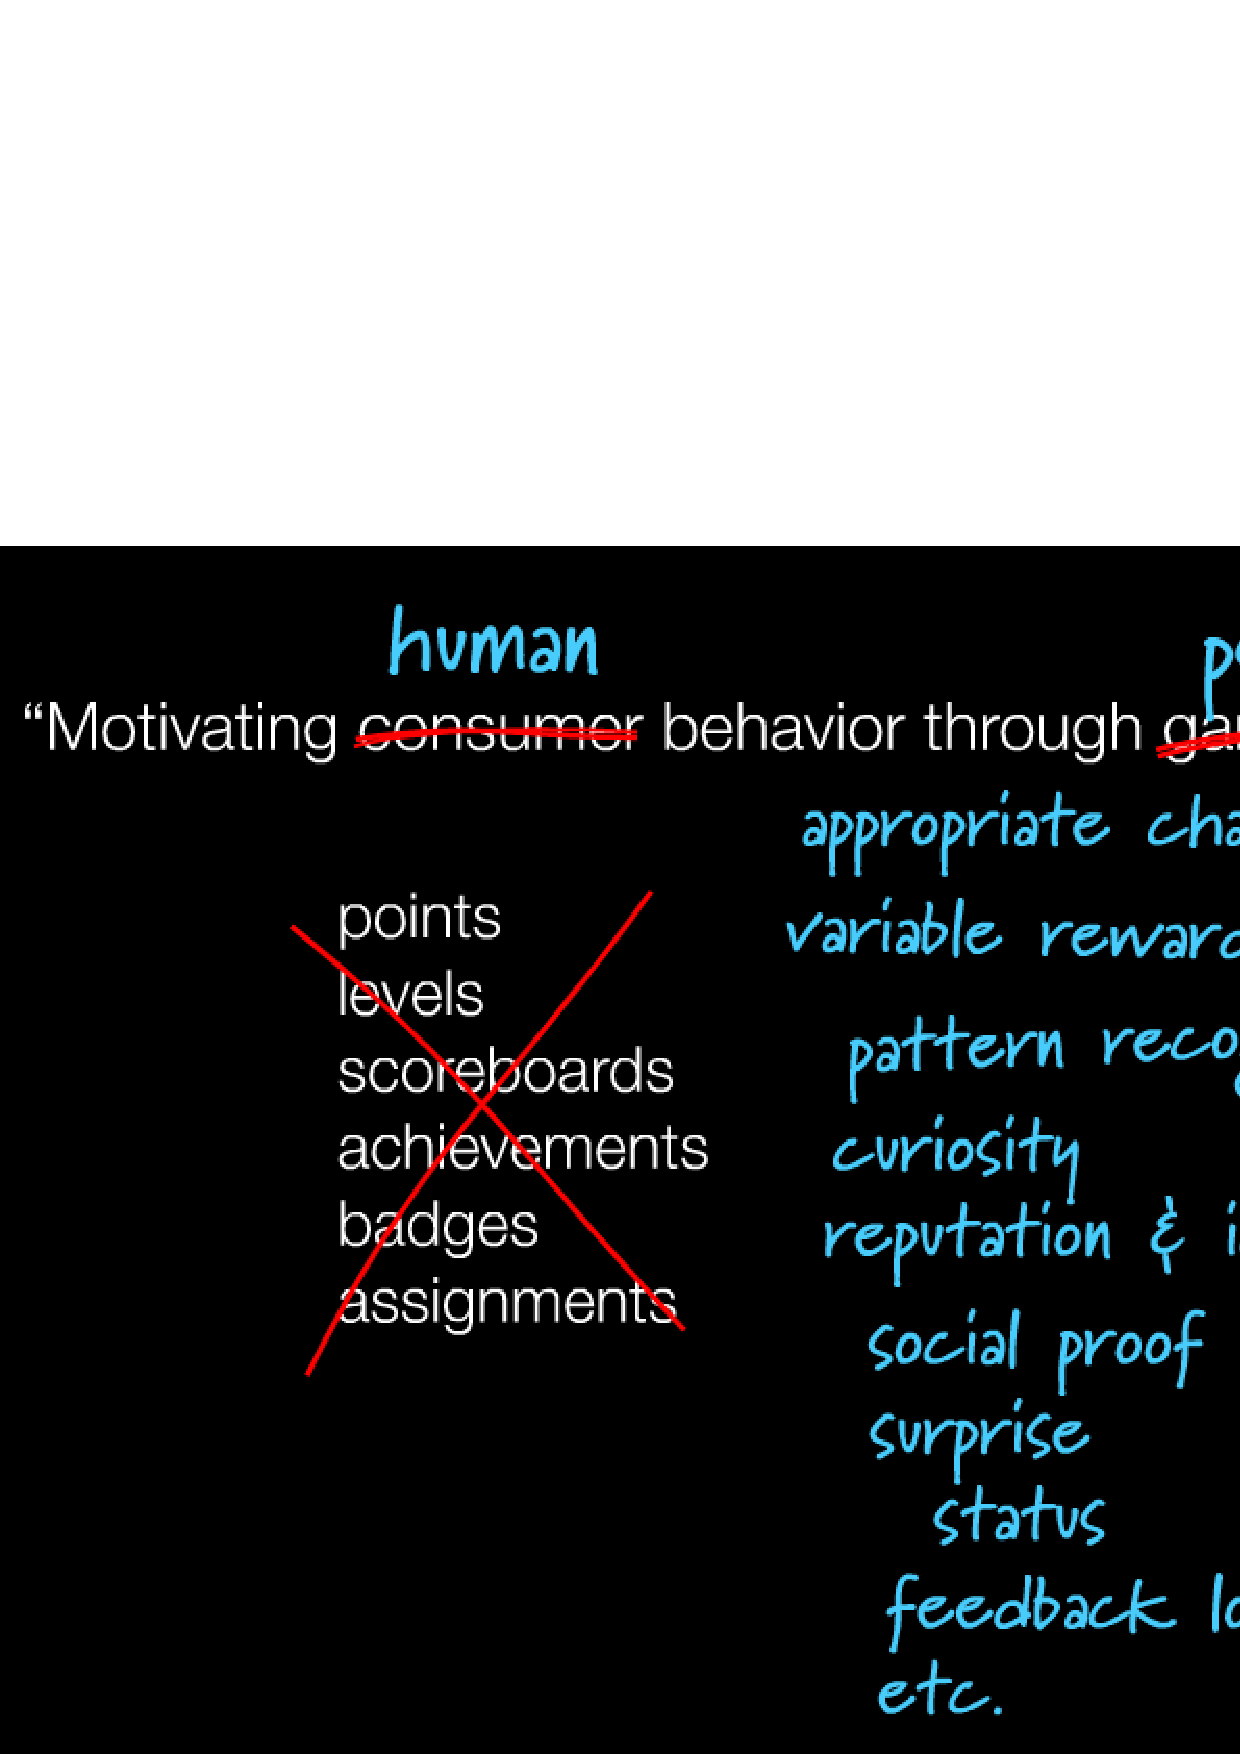
\includegraphics[scale=0.25]{anti-gamification.png}
		\caption{Gamification is about extrinsic rewards (source: Anderson \cite {anderson2011})}
		\label{fig:anti-gamification}
\end{figure}

Although Jane McGonigal is the advocate of employing games in reality, she spoke about her concern about current state of gamification in the GDC 2011 talk titled ``We don�t need no stinking badges: How to reinvent reality without gamification'' \cite {mcgonigal2011}. She argued that current gamification confuses intrinsic/extrinsic motivation and proposed ``Gameful Design'' instead of ``Gamification''. She claimed that "Gameful is player-oriented", which presumed that the loyalty program type gamification is product or service oriented. While the current gamification is about extrinsic reward, with points, badges, and levels, gameful design is about intrinsic reward, with positive emotion, relationships, meaning and accomplishment.

The followings are a few more eminent criticisms of gamification:

\subsection{Gamification is Bullshit}
Georgia Institute of Technology professor and game designer Ian Bogost called gamification efforts ``exploitation-ware" that is being ``invented by consultants'' and claimed that gamification is bullshit \cite {bogost}. Gamification, he argued, ``gets games wrong, mistaking incidental properties like points and levels for primary features like interactions with behavioral complexity". In the GDC 2011 gamification debate, he contrasted that ``To take something like games, which are complicated, and substitute it out for points and badges is a very efficient way to get a hot culture commodity into your product" \cite {magrino2011}. 

\subsection{Gamification vs. Poinstification}
In her blog, game designer Margaret Robertson stated that current gamification is the wrong word for the right idea. ``What�s happening at the moment is Pointsification'' \cite {robertson2010}. She criticized that
the current use of gamification is a bad thing because it�s a misleading title for a misunderstood process. Points and badges are the least important bit of a game. She also pointed out: ``Pointsification is a perfectly valid and valuable concept which nonetheless needs to be implemented carefully with due concern for appropriateness and for unintended consequences''.

\subsection{Intrinsic vs. Extrinsic Motivation}
Many considered the current efforts of gamification focus on extrinsic motivators (such as points, badges and rewards) instead of intrinsic motivators generated by an individual's internal will or desires. 

Nicole Lazzaro argued that the use of extrinsic rewards will decrease the motivation to use your products and services once you remove that reward \cite {Lazzaro2011}. Vockell resonated that in education psychology, extrinsic motivators may lead to short-range activity increase but reduction in long-range interest in a topic. While intrinsic motivators motivate people best when they are working toward personally meaningful goals \cite{vockell2004educational}. 

Michael Wu argues that extrinsic rewards can jumpstart intrinsic motivation  \cite {WuSustainable2011}. He claimed that gamification just has to work long enough for some other processes to take over as the primary driver of value. Subsequently, it becomes a secondary reinforcement system. 

\section{Gamification Design}
This section describes the current approach in gamification design. It starts with gamification design 1.0 with simply adding point, badge and leader board in applications. In the end it discusses the smart gamification that emphasizes a player's journey to mastery in an application.

\subsection{Gamification 1.0}
Different game mechanics and elements can be used to serve different functions in satisfying players' needs, and the basic elements such as point, badge, and leader board are the defining attributes of the current gamification practices \cite {Deterding2011dragon}.

\begin{figure}[htbp]
	\centering
		\subfigure[Satisfies Human Needs (source: Bunchball)]{\label{fig:human-needs}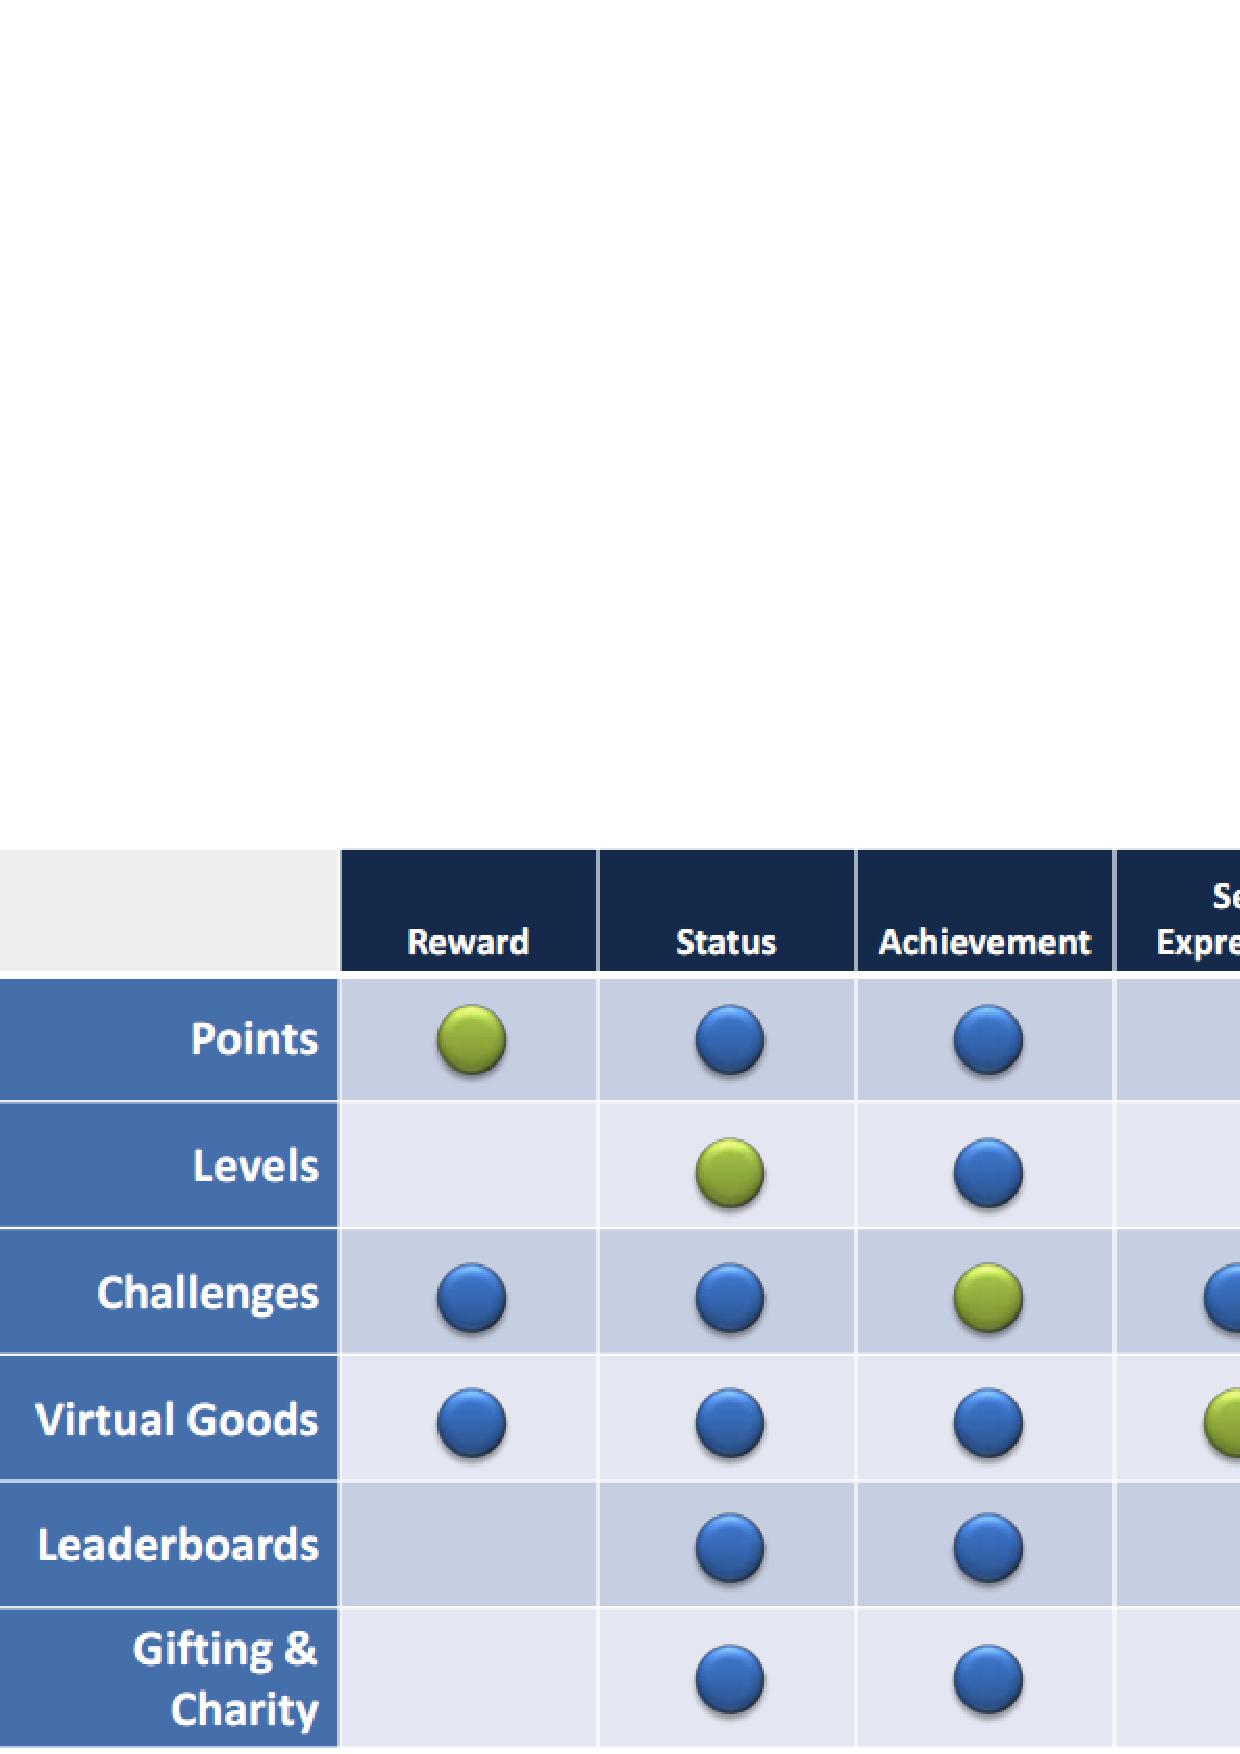
\includegraphics[width=3.2in]{human-needs.png}}
		\subfigure[Basic Mechanics (source: Deterding \cite{Deterding2011meaningful})]{\label{fig:basic-elements (source: }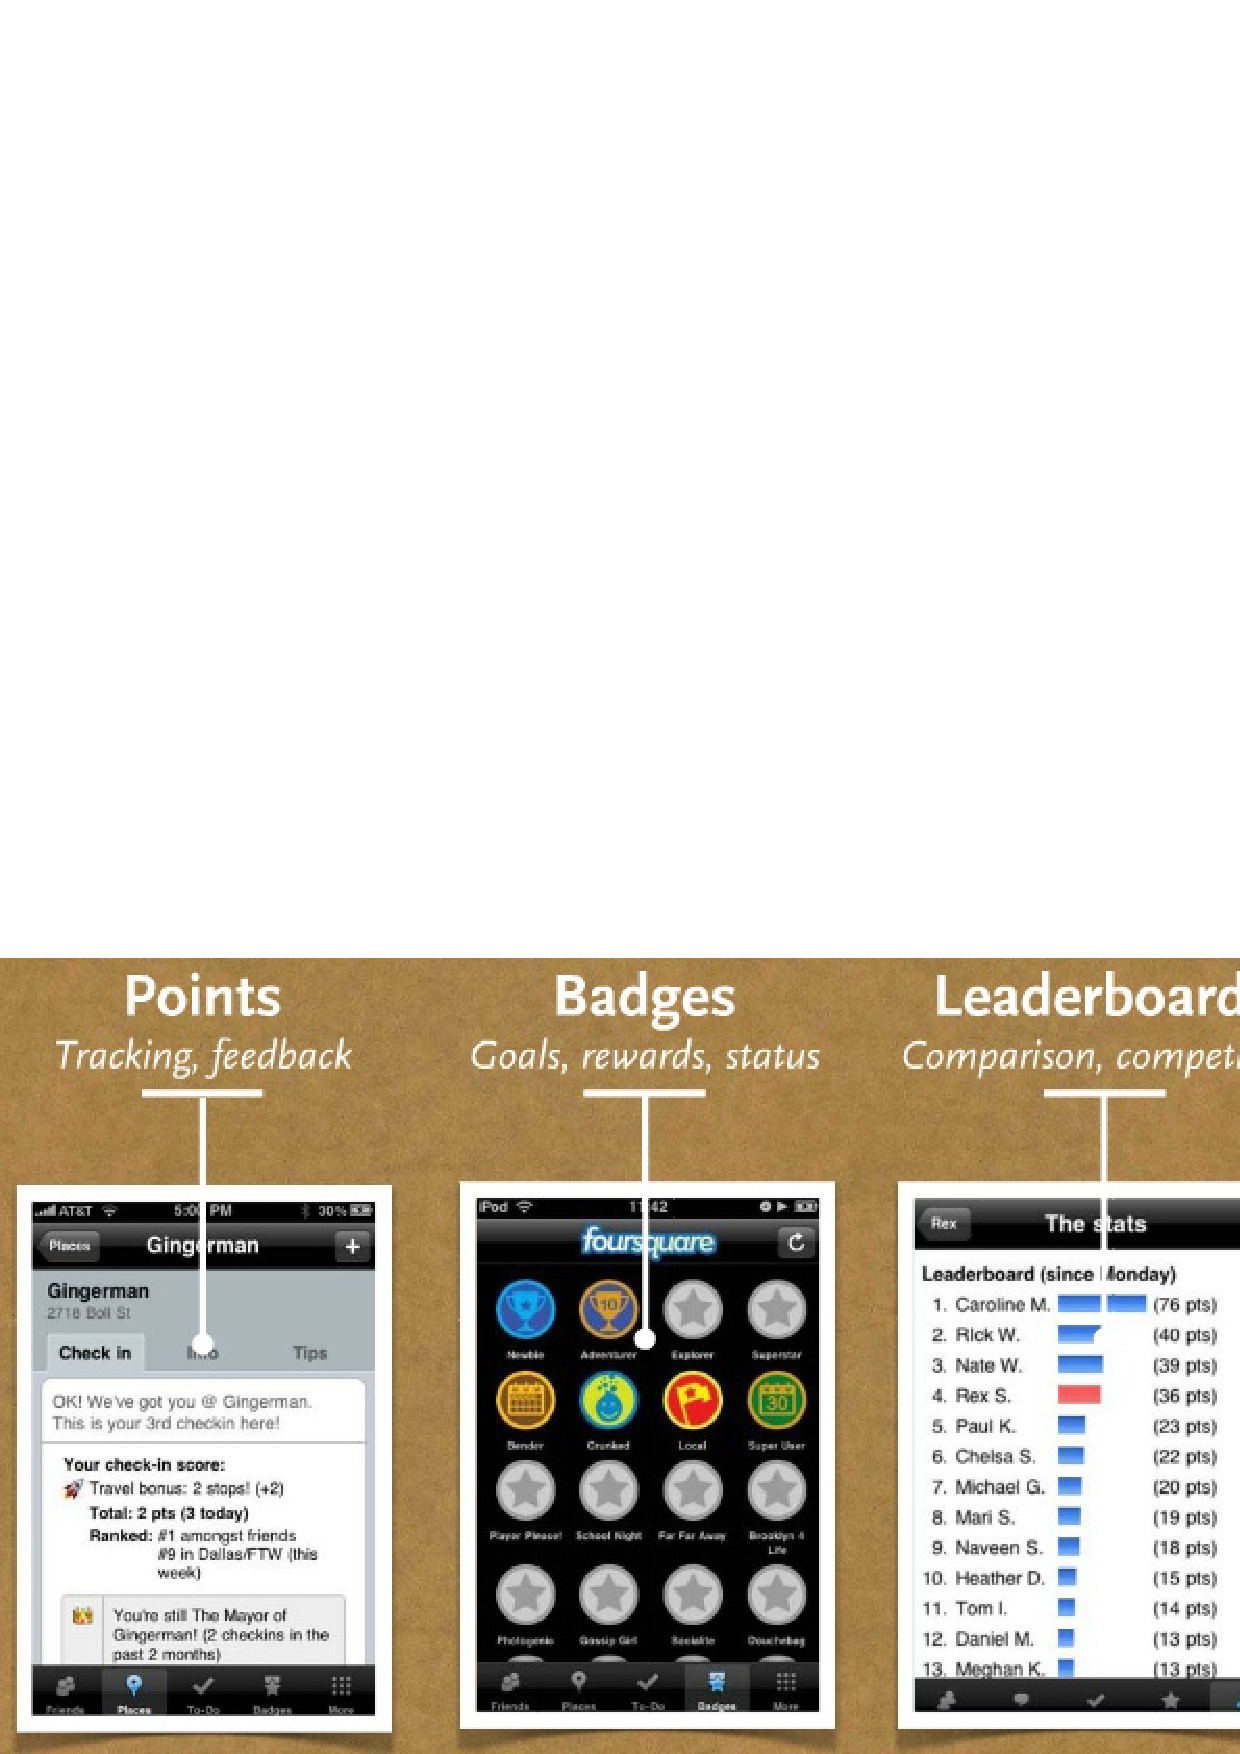
\includegraphics[width=3.2in]{basic-element.jpg}}
		\caption{Gamification 1.0}
		\label{fig:gamification-1-0}
\end{figure}

\subsection{List of Game Mechanics and Elements}
Seth Priebatsch stated that you can get anyone to do anything with seven game dynamics \cite {Priebatsch2010ted}. Techcrunch published a ``secret'' game dynamics play deck that is used by Priebatsch's company SCVNGR \cite{Biggs2010}. The play deck is a set of 47 flash cards. Each card illustrates one game dynamics. SCVNGR employees are instructed to memorize them and apply in their applications as needed.  Social interaction designer Adrian Chan posted a blog, "I just killed a social game mechanic" \cite {Chan2010}, commented on each of the deck�s 47 points. He also noted that the sociological factors in social gaming are not listed in the deck and the play deck confuses game mechanics and game dynamics. 

Gamification.org compiles a list of game mechanics and categories them into three types (Behavioral, Feedback, Progression) and their benefits \cite{gamificationwiki}. Table 2.3 - 2.5 organizes the mechanics in type, a short description or examples, benefits, and possible player types in Bartle's model \cite {bartle1996hearts}:

\begin{table}[htbp]
  \centering
    \caption{List of Game Mechanics}
    \begin{tabular}{ | l | p {6cm} | p {4cm} | p {2cm} |}
    \hline
    \bf{Types} & \bf{Mechanics / Examples} & \bf{Benefits} & \bf{Player Types} \\ \hline
	Progression & Achievements: normally represents as badge, completed something & Engagement, Loyalty, Time Spent, Influence, Fun, SEO, UGC & Achievers, Explorers, Killers \\ \hline
	Progression & Levels: a system of reward for a cumulation of points, Often are unlocked as players progress to higher levels. & 	Engagement, Loyalty, Influence, Time Spent, Virality, Fun & Achievers, Explorers, Killers \\ \hline
	Progression & Points: a running numerical value given for any single action or combination of actions. & Engagement, Loyalty, Influence, Time Spent, Virality, Fun, UGC & Achievers, Explorers, Killers \\ \hline
	Progression & Progression: success is granularly displayed and measured through the process of completing itemized tasks, such as a progress bar. & Engagement, Loyalty, Influence, Time Spent, Fun, UGC & Achievers, Killers \\ \hline
	Feedback & Appointment Dynamics: at a predetermined times/places a user must return for a positive effect & Engagement, Influence, Time Spent & Archivers, Explorers, Socializers \\ \hline
	Feedback & Bonuse: a reward after having completed a series of challenges or a specific task & Engagement, Influence, Time Spent, Virality, Fun, UGC & Archivers, Explorers, Socializers, Killers \\ \hline
    \end{tabular}
\end{table}

\begin{table}[htbp]
  \centering
    \caption{List of Game Mechanics (cont.)}
    \begin{tabular}{ | l | p {6cm} | p {4cm} | p {2cm} |}
    \hline
     \bf{Types} & \bf{Mechanics / Examples} & \bf{Benefits} & \bf{Player Types} \\ \hline	
	Feedback & Cascading Information Theory: information should be released in the minimum possible snippets to gain the appropriate level of understanding & Engagement, Loyalty, Influence, Time Spent & Archivers, Explorers, Socializers, Killers \\ \hline
	Feedback & Combos: reward skill through doing a combination of things, usally comes with the reward of a bonus & Engagement, Influence, Time Spent, Virality & Archivers, Explorers, Socializers, Killers \\ \hline
	Feedback & Countdown: players are only given a certain amount of time to do something. This will create an activity graph that causes increased initial activity increasing frenetically until time runs out, which is a forced extinction. & Engagement, Fun, Influence & Achievers, Explorers, Killers \\ \hline	
	Feedback & Quests/Challenges: Challenges usually implies a time limit or competition whereas Quests are meant to be a journey of obstacles a player must overcome. a way to organize player effort. & Engagement, Loyalty, Revenue, Influence, Time Spent, Virality, SEO, Fun, UGC & Achievers, Explorers, Killers \\ \hline
	Feedback & Reward Schedules: The fixed or variable timeframe and delivery of the rewards, contingency, response, reinforcer. & Engagement, Loyalty, Revenue, Influence, Time Spent, Virality, SEO, Fun, UGC & Achievers, Explorers, Killers \\ \hline
	Behavioral & Discovery/Exploration: players love to discover and to be surprised. & Engagement, Loyalty, Influence, Time Spent, Fun & Explorers, Achievers \\ \hline
	Behavioral & Epic Meaning: Players will be highly motivated if they believe they are working to achieve something great, something awe-inspiring, something bigger than themselves. & 	Engagement, Loyalty, Influence, Time Spent, Fun & Achievers, Explorers, Socializers, Killers \\ \hline
    \end{tabular}
\end{table}

\begin{table}[htbp]
  \centering
    \caption{List of Game Mechanics (cont.)}
    \begin{tabular}{ | l | p {6cm} | p {4cm} | p {2cm} |}
    \hline
     \bf{Types} & \bf{Mechanics / Examples} & \bf{Benefits} & \bf{Player Types} \\ \hline	
	Behavioral & Free Lunch: getting something for free due to someone else having done work. Groupon & Engagement, Loyalty, Revenue, Influence, Virality, Fun & Achievers, Explorers,  Socializers, Killers \\ \hline
	Behavioral & Infinite Gameplay: do not have an explicit end, static state is its own victory. & 	Engagement, Loyalty, Revenue, Influence, Time Spent, Fun & Achievers, Killers \\ \hline
	Behavioral & Loss Aversion: influences user behavior not by reward, but by not instituting punishment. the player having to perform an action to avoid losing something they currently have. & Engagement, Loyalty, Influence, Time Spent, Virality, Fun & Achievers, Explorers \\ \hline
	Behavioral & Lottery:  the winner is determined solely by chance. winners will generally continue to play indefinitely while losers will quickly abandon & Engagement, Loyalty, Revenue, Influence, Time Spent, Virality, Fun & Achievers, Explorers, Socializers, Killers \\ \hline
	Behavioral & Ownership: creates Loyalty by owning things. & Engagement, Loyalty, Revenue, Influence, Time Spent, Virality, SEO, Fun, UGC & Achievers, Explorers, Socializers, Killers \\ \hline
	Behavioral & Community Collaboration: an entire community is rallied to work together to solve a riddle, a problem or a challenge. Immensely viral and very fun. & 	Engagement, Influence, Time Spent, Virality & Archivers, Explorers, Socializers \\ \hline
    \end{tabular}
\end{table}

\begin{table}[htbp]
  \centering
    \caption{List of Game Mechanics (cont.)}
    \begin{tabular}{ | l | p {6cm} | p {4cm} | p {2cm} |}
    \hline
     \bf{Types} & \bf{Mechanics / Examples} & \bf{Benefits} & \bf{Player Types} \\ \hline	
	Behavioral & Behavioral Momentum: a tendency of players to keep doing what they have been doing & Engagement,  Loyalty, Revenue, Influence, Time Spent & Archivers, Explorers, Socializers, Killers \\ \hline
	Behavioral & Blissful Productivity: playing hard rather than relaxing makes you happier  & Engagement & Archivers, Explorers, Socializers, Killers \\ \hline
	Behavioral & Status: The rank or level of a player. Players are often motivated by trying to reach a higher level or status. Also relates to envy. & Engagement, Loyalty, Revenue, Influence, Time Spent, Virality, SEO, Fun, UGC & Achievers, Socializers,Killers \\ \hline
	Behavioral & Urgent Optimism: The desire to act immediately to tackle an obstacle combined with the belief that we have a reasonable hope of success. & Engagement, Fun & Explorers, Killers \\ \hline
	Behavioral & Virality: more successful in the game if you invite your friends, the social check-in. & Engagement, Loyalty, Revenue, Virality, SEO, UGC & Socializers, Achievers,Killers \\ \hline
    \end{tabular}
\end{table}

Game Elements are different than mechanics. They manifest the game information to the player, usually as UI components. Table 2.6 lists some popular game elements and their examples:

\begin{table}[htbp]
  \centering
    \caption{List of Game Elements}
    \begin{tabular}{ | l | p {12cm} |}
    \hline
    \bf{Elements} & \bf{Description and Examples} \\ \hline
	Activity Feed & shows players what has been taking place in the system overall and motivate the player to obtain the same achievement as others. \\ \hline
	Avatars & unique representations for a player. shows a high emotional attachment between the player and the game. often customization and decoration are enhancement for higer engagement. \\ \hline
	Easter Eggs & an intentional hidden message, in-joke. \\ \hline
	Instances & are created for players to have a unique experience that is outside the normal experience. When a player creates a special unique page experience that allows to log into and view their unique content an instance has been created. \\ \hline
	Leader boards & are a means by which users can track their performance, subjective to others. Leaderboards visually display where a user stands in regards to other users. Leaderboards can be broken down into several subcategories such as: Global, Friends, Relative, Isolated etc. \\ \hline
	The Notifier & is a direct way to give the user direct feedback about their progress, change of status in the gameplay experience etc. \\ \hline
	User Profile & displays a User's data about their activity on a website and can be used to tell the world and a community on the internet who they are. \\ \hline
    \end{tabular}
\end{table}

\subsection{Four Keys to Fun}

By doing a research study of 15 hardcore gamers, 15 casual games, and 15 non-players, Nicole Lazzaro identified the four Keys to releasing player's emotions during play: "Hard Fun, Easy Fun, Serious Fun, and People Fun" \cite {lazzaro2004we}. Most of the popular games selected in their research created emotion in at least three of the Four Keys, thus she suggested that combining these four keys in the game design will make a deeply enjoyable game for a wide market.

Nicole Lazzaro described the ``Four Keys to Fun'' framework to design better engagement in games, especially the MSO (Massively Social Online) games \cite{Lazzaro2011}.

\begin{figure}[htbp]
	\centering
		\includegraphics[scale=0.7]{4k2fchasingwondermap.jpg}
		\caption{Four Keys to Fun Game Map}
		\label{fig:four-keys-to-fun}
\end{figure}

\subsection{Game Design Frameworks}

Game designer Marc LeBlanc introduced the popular game design framework ``Mechanics / Dynamics / Aesthetics(MDA)'' which describes three pillars of a good game \cite {hunicke2004mda}: 

1. Mechanics: the various actions, behaviors and control mechanisms afforded to the player within a game context. They make up the functioning components of the game.

2. Dynamics: run-time behavior of inputs and outputs between player and game, They are the player's interactions with mechanics.

3. Aesthetics: The desirable emotional responses evoked by the game dynamics. They are how the game makes the player feel.

\subsection{Smart Gamification}
Amy Jo Kim presented ``Smart Gamification'' which focuses on designing the effective ``Player Journey'' with intrinsic reward preferred over extrinsic reward \cite {Kim2010}. Kim pointed out that game techniques are not equal to core experience and intrinsic values are greater than extrinsic rewards. Kim stated that ``a good game take the player on a journey toward mastery". When overtime players experience from newcomer and become regular and finally turns into enthusiast, they progress from novice to expert and last to master. When designing the journey, Kim suggests to use different techniques to meet players needs, where  novices need onboarding, experts need fresh content, activities and challenges, and masters need exclusivity, recognition and impact. Kim incorporates the MDA framework, using it to guide and motivate the player journey.

\begin{figure}[htbp]
	\centering
		\subfigure[Player Lifecycle]{\label{fig:player-lifecycle}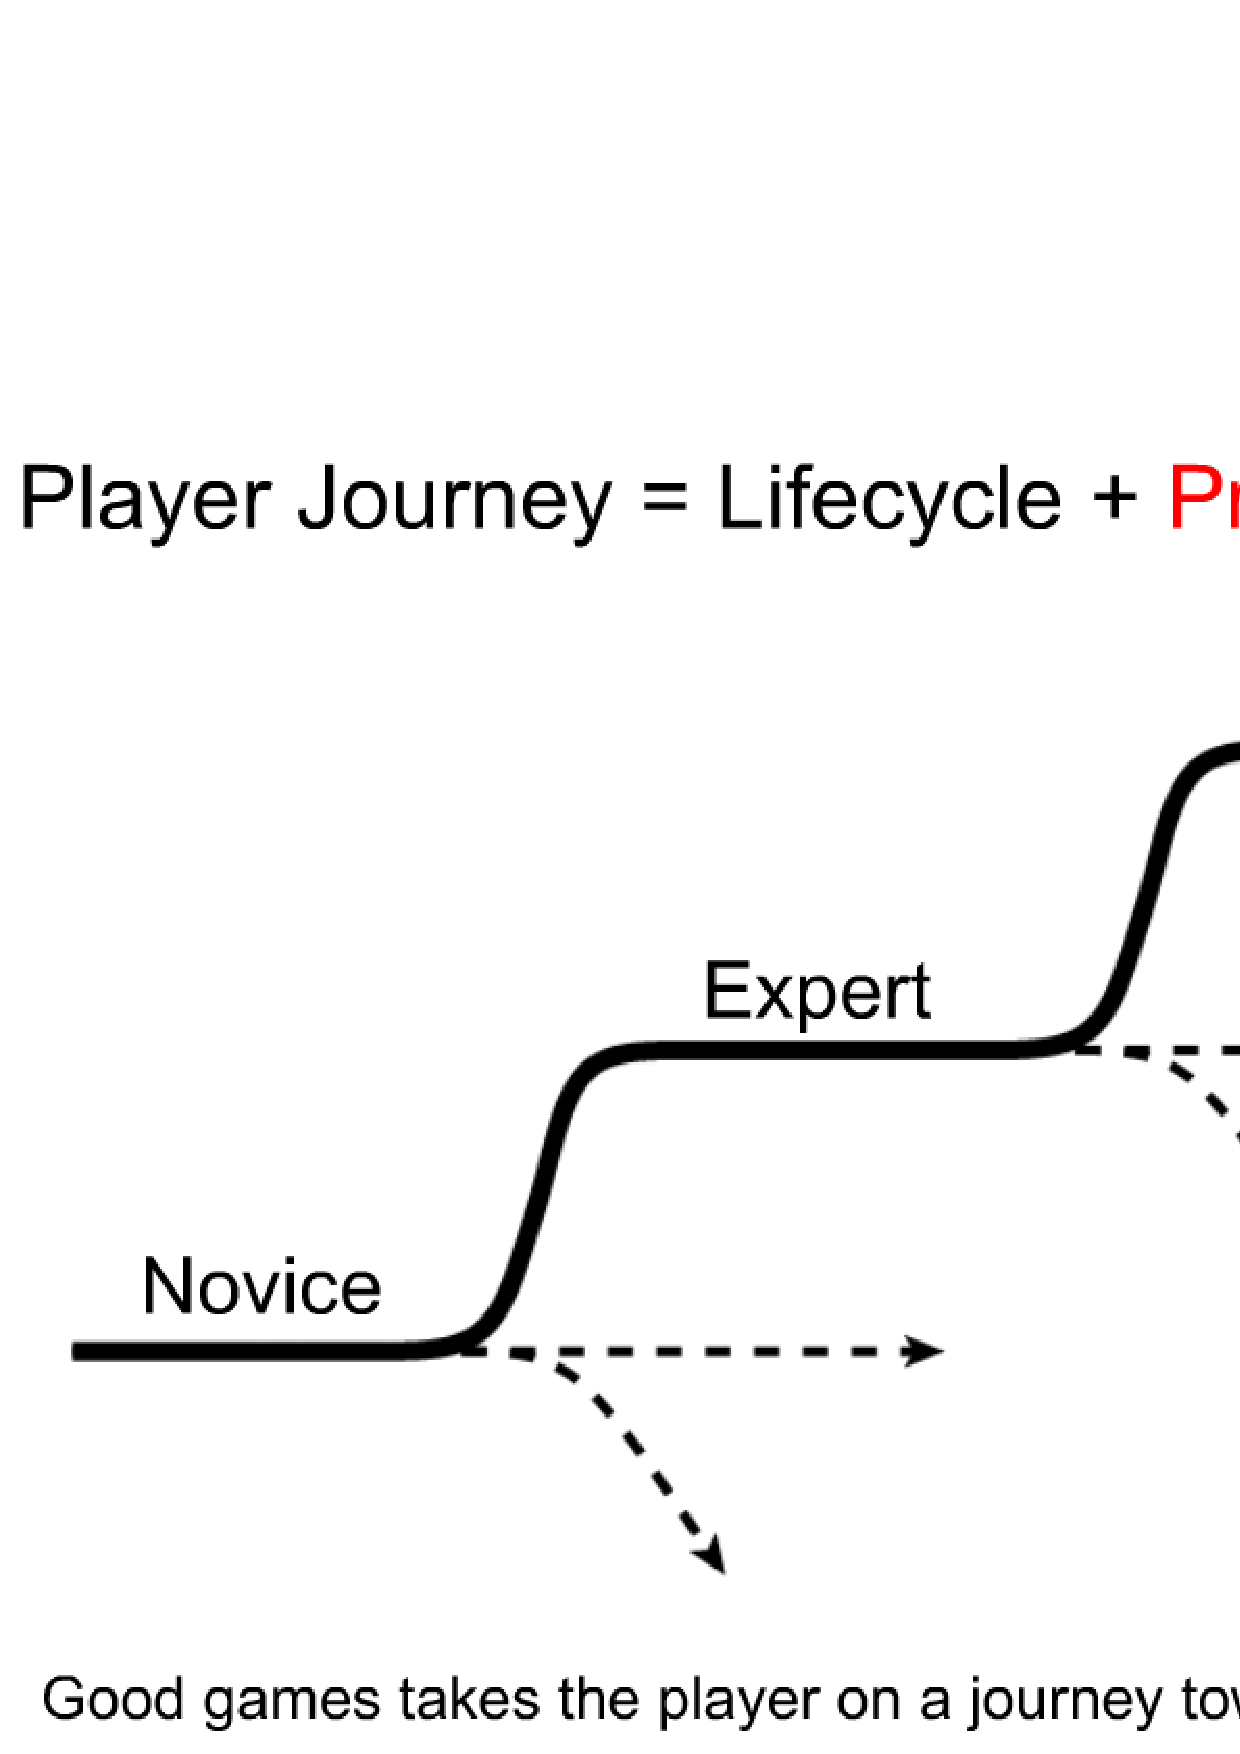
\includegraphics[height=2in]{kim-workshop.png}}
		\subfigure[Game Design]{\label{fig:game-design}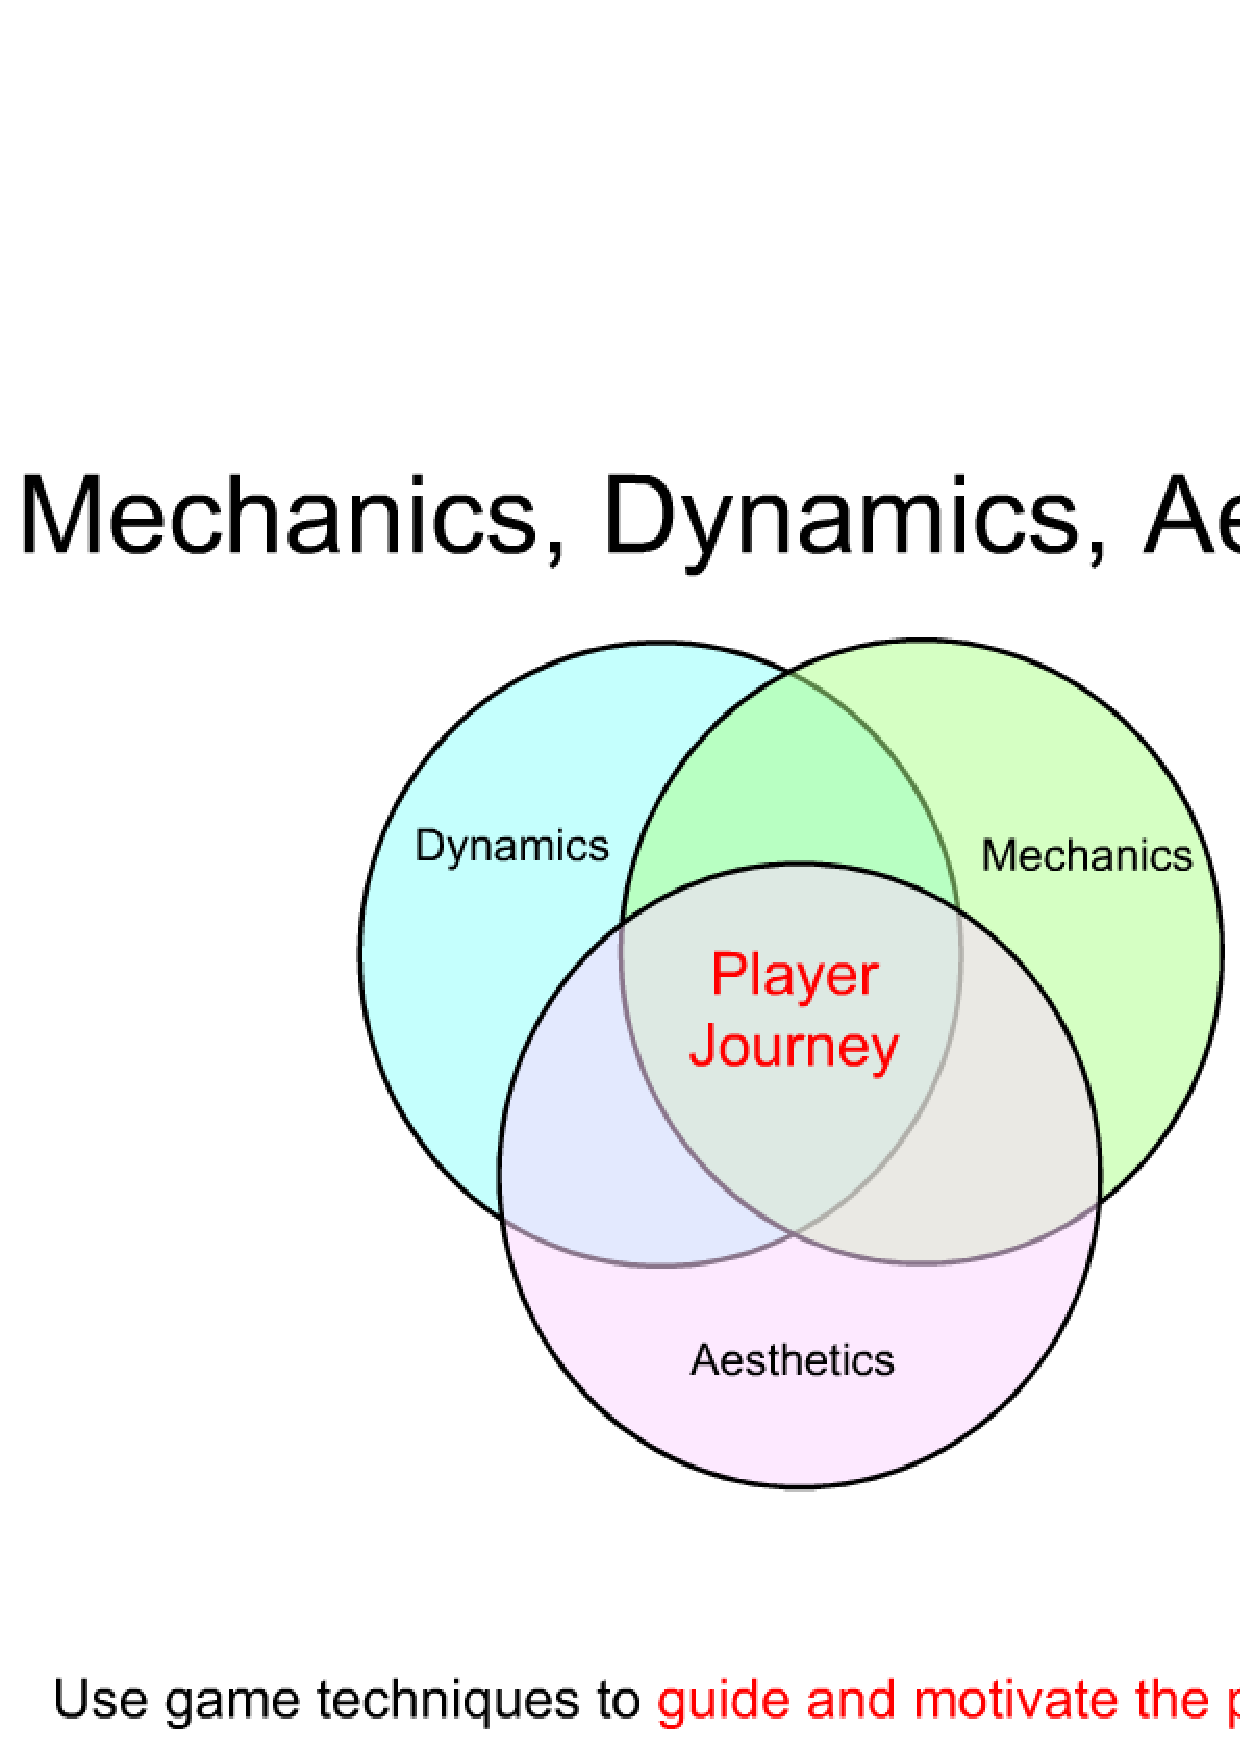
\includegraphics[height=2in]{kim-workshop2.png}}
		\caption{Designing Player Journey (source: Kim \cite {Kim2010})}
		\label{fig:design-player-journey}
\end{figure}

Similarly, researcher Sebastian Deterding not only criticized the current practice of simple gamification practices but stressed the important of ``meaningful play'' and proposed a user experience design around the three most important aspects: Meaning, Master and Autonomy \cite {Deterding2011meaningful}. It is an adaptation to the three elements to motivate people in Daniel Pink's book "Drive: The Surprising Truth About What Motivates Us" \cite {pink2009drive}. Deterding explained that the reason why we play is because of the meaning and autonomy with choice in the game. The mastery in the game give us fun and enjoyment.

\section{Gamification Services and Platforms}
There are several gamification services and platforms from by commercial companies and open source providers. They aim to meet the increasing needs of gamifying non-game applications.

\subsection{Commercial products and services}
This section outlines the current industry players that provide gamification services via platforms or consultation services, as illustrated in Figure 2.14. Almost all of them are recent startups funded by venture capitals.

\begin{figure}[htbp]
	\centering
		\includegraphics[scale=0.4]{gamification-service.pdf}
		\caption{Gamification Service Industry}
		\label{fig:gamification-service}
\end{figure}

Here we take a brief look at the three most active players:

{\bf Badgeville} \cite {badgeville} brands itself to be the world's leading Social Loyalty Platform. Its products include "Dynamic Game Engine", providing an easy and flexible way to setup behaviors, rewards, missions; "Gamification Widget Studio", offering a collection of skinnable and configurable game mechanics widgets; "Social Fabric", integrating social graph, social notification, relevant activity streams for better social engagement. 
    
{\bf Bunchball}'s \cite {bunchball} Nitro Platform provides a comprehensive set of game mechanics, besides the normal points and badges levels, it provides Actions, Groups, Virtual Goods, Social networks, Trivia, Poker, Comments etc. It is a fully integrated platform for engineers, designers, and marketers. Another product that Bunchball introduced is the Nitro Elements, which is a suite of cloud-based, simple plug and play applications, that is aimed for quick implementation of gamification. The current elements includes "FanBox" (a reward system) and "GameBox" (hosted poker game).

{\bf BigDoor}  \cite {bigdoor} also provides a platform with flexible API and customizable widgets to add game mechanics to web sites, to reward users with points, badges, achievements and leader boards. The javascript based "MiniBar" widget is a quick way to add game layer to the web site. 

All of the above platforms feature built-in analytics built to provide some kinds of  metrics about the result of the gamification. While Badgeville seems emphasize on social integration; Bunchball provides a comprehensive solution even with a game box; and BigDoor provides a simplest "MiniBar" for easy non-technical integration into existing web site.

\subsection{Mozilla - Open Badges Infrastructure}

Open Badges \cite {openbadges}  is a project of Mozilla with support from the MacArthur Foundation to provide a software infrastructure to making it easy to issue and display badges across the web. It uses shared badges as the recognition for all types of learning and achievement that take place anywhere, such as a skill learned from after-school program, a certification earned or simply an achievement of providing useful technical answers. The badges could be displayed in the personal or social web site, or being used in the job search as a convenient showcase of applicant's qualification.

\begin{figure}[htbp]
	\centering
		\includegraphics[scale=0.4]{open-badge.jpg}
		\caption{Mozilla - Open Badges Infrastructure}
		\label{fig:open-badge}
\end{figure}

\subsection{Open Source Gamification Platform}
Userinfuser \cite {UserInfuser}  is an open source platform that provides customizable gamification elements designed to increase user interaction on web sites. The project involves badging, points, live notifications, and leader boards. Additionally, the platform provides analytics to track user participation. The current documentation shows the following widgets available in the platform. 

\begin{figure}[htbp]
	\centering
		\includegraphics[scale=0.4]{userinfuser.jpg}
		\caption{Open Source Gamification: Userinfuser Widget}
		\label{fig:userinfuser}
\end{figure}

\section{Related Concepts}

\subsection {Serious Game}
A Serious game is a game designed for a primary purpose other than pure entertainment (Wikipedia). It includes categories such as educational games and advergames (advertising), political games, and training game (also known as game-learning).

One excellent example is Fold.it, which made the headline \cite {khatib2011crystal} by using game play to help solve problems that computers cannot solve very well, in this case, online gamers were able to do what biochemists have been trying to do for a decade: decipher the structure of a protein that is key to the way HIV multiplies.

The difference between Gamification and Serious game is not very clear. Both are trying to solve a problem with game thinking. Some reference serious game such as Foldit as a victorious example of gamification in science \cite{bosch2011}. Sebastian Deterding's definition \cite {Deterding2011mt}  illustrates that gamification are total different than serious game.

It is interesting to see that although the concept of serious games has been around since long before gamification, gamification has arguably steps into the mainstream whereas serious games stay in much smaller scale.  

\subsection{Persuasive Game}
The term "Persuasive game" is introduced in the title book "Persuasive Games, The Expressive Power of Video games" by Ian Bogost \cite {bogost2007persuasive}. In the book, Bogost argues that video games have a unique persuasive power that goes beyond other forms of computational persuasion. Not only can video games support existing social and cultural positions, as in Serious games, but they can also disrupt and change those positions, leading to potentially significant long-term social change, as in Persuasive games.

Persuasive game is closely tied to Persuasive Technology, designed to change attitudes or behaviors of the users through persuasion and social influence, but not through coercion \cite {fogg_2003}.

Loren Baxter \cite {baxter_2011} posted that persuasive design, the use of psychology in design to influence behavior, could benefit UX design in a new level, hinting the use in gamification design as well.

\subsection{Gameful Interaction Design}
According to The Interaction Design Association (IxDA) \cite {Wroblewski},
Interaction design defines the structure and behaviors of interactive products and services, and user interactions with those products and services. It is design principle with main focus on behavior. \cite {norman2002design}. 

For example, the "SmartGauge" dashboard for Ford's hybrid cars, where a digital plant is responding to how energy-efficient the users driving behavior is \cite {ideo2009}. The design gives drivers a game like interaction that for them, the game to grow more lush and beautiful leaves, a visual reward, by driving efficiently, desired behavior. 

Another great example is the "Piano Staircase" created by Volkswagen Sweden and ad agency DDB, installed in a metro station in Stockholm \cite {funtheory2009}. The design is to make the staircase next to the escalator look and respond like a piano keyboard, so that every step on the stair will generate different piano sounds every time a commuter walked on it. Observation indicates that 66 percent more people chose the staircase over the escalator, a good example of a "Fun Theory" design for persuading and encouraging energy-efficient behavior.

 \begin{figure}[htbp]
	\centering
		\subfigure[Efficiency Leaves]{\label{ixd-dashbard}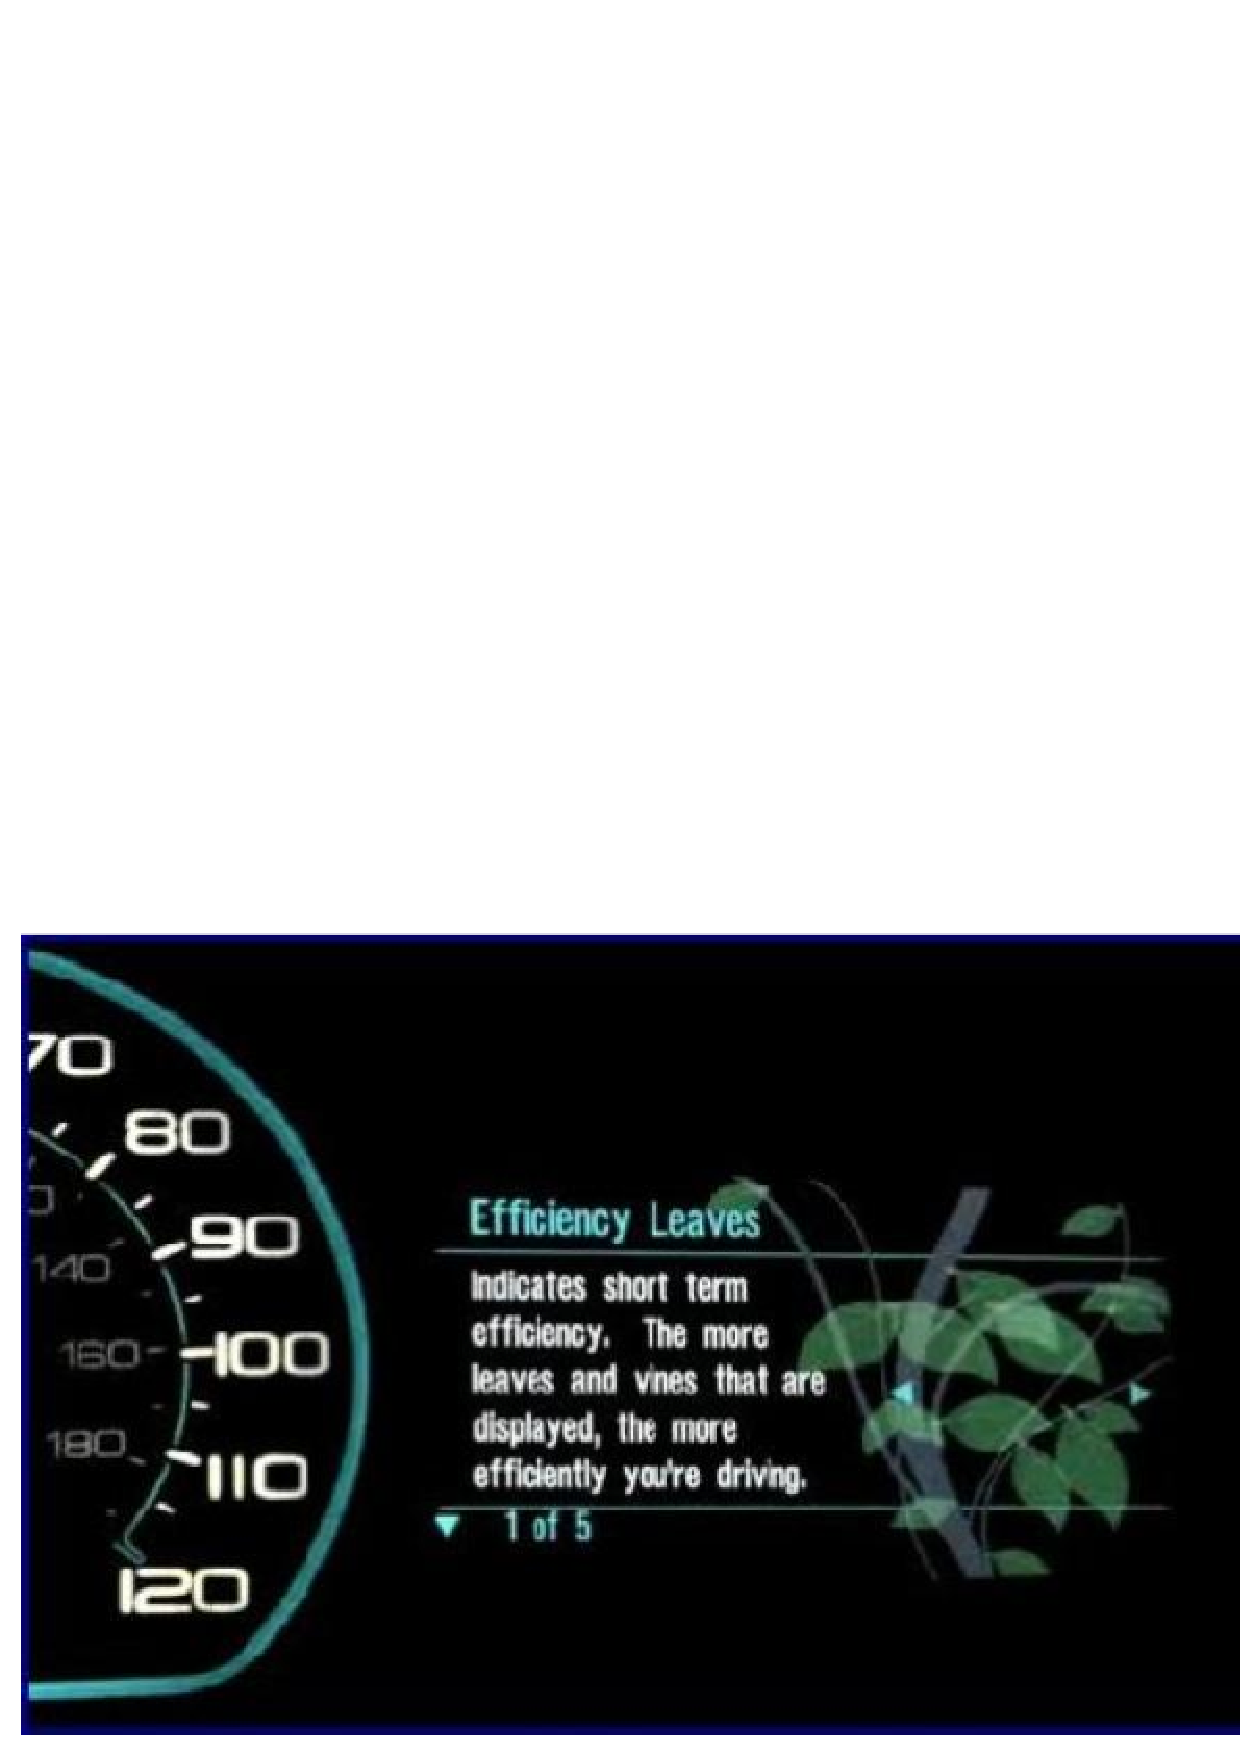
\includegraphics[scale=0.3]{ixd-dashboard.png}}
		\subfigure[Piano Stair vs. Escalator]{\label{fig:ixd-pianostair}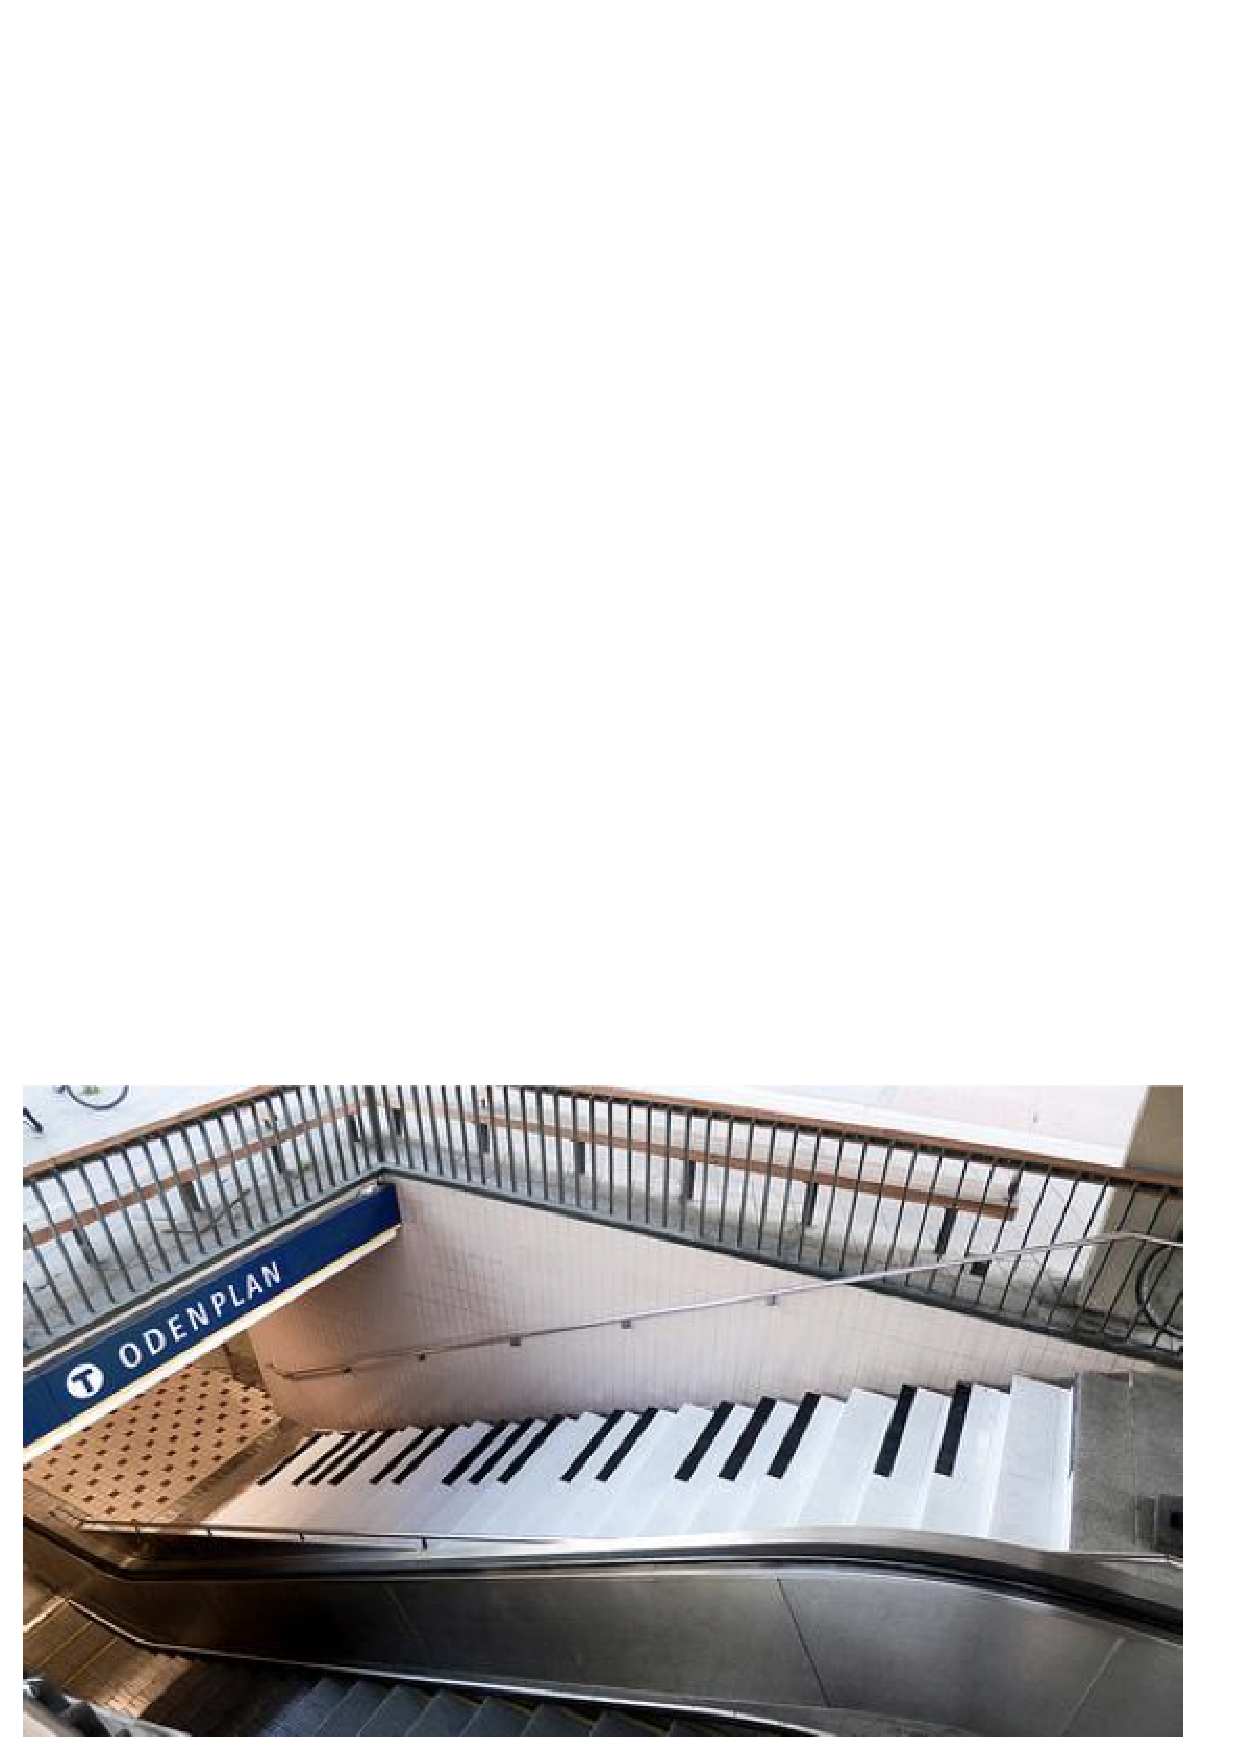
\includegraphics[scale=0.35]{ixd-pianostair.png}}
		\caption{Examples of Gameful Interaction Design}
		\label{fig:ixd}
\end{figure}	

The goal of such gameful interaction design is to achieve a certain influence, a change in the behavior of their users not through a mode of informative feedback and rational processing, but through the activation of emotion or sensibility. 

\section{Gamification Analytics}

Ducheneaut and Yee etc provides a good example of 
using game metrics for analysis of player's experience in a quantitative approach \cite {ducheneaut2006alone}. They reported the relationship of playing time and leveling in the MMORGs, as shown in Figure 2.18:

\begin{figure}[htbp]
	\centering
		\subfigure[Average time required to reach a level]{\label{fig:metrics1}
\includegraphics[height=1.7in]{metrics1.png}}
		\subfigure[Average accumulated play time by level]{\label{fig:metrics2}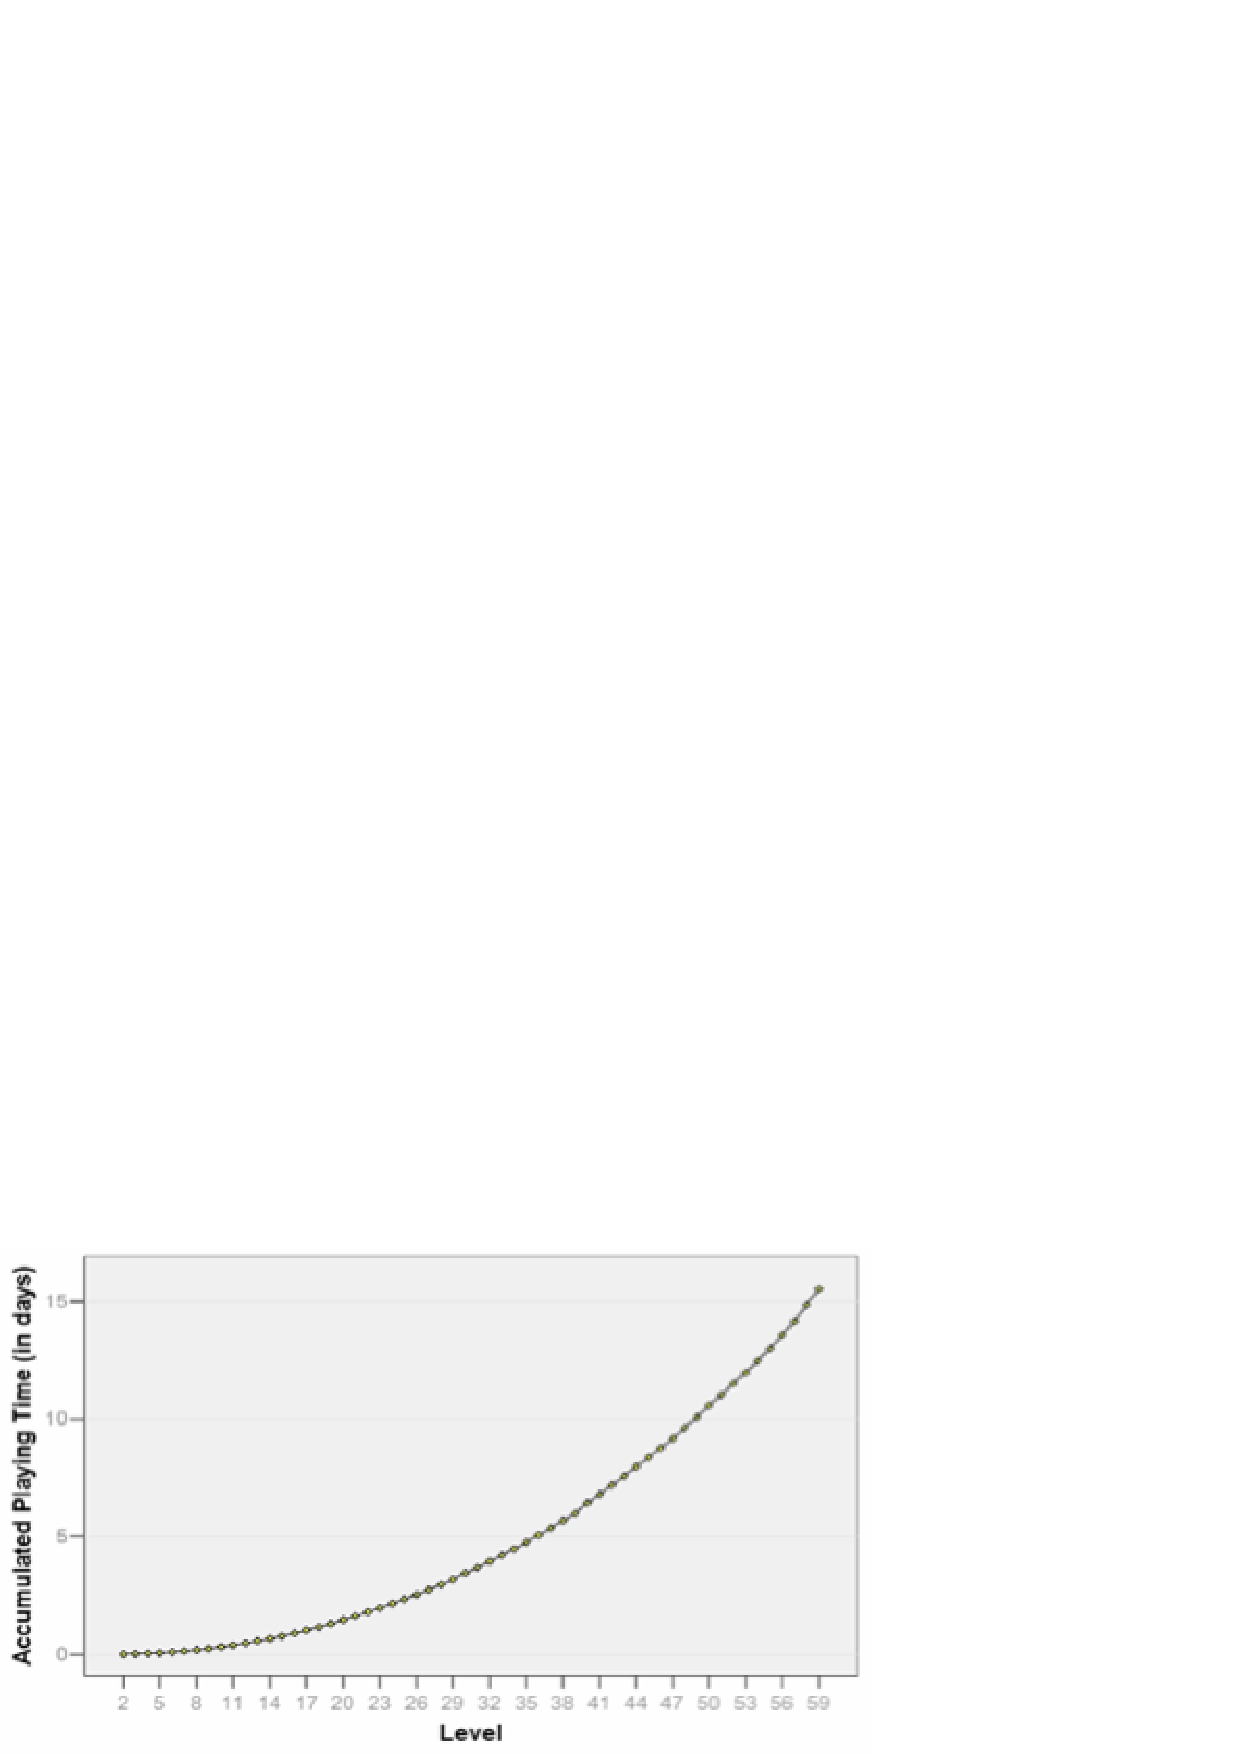
\includegraphics[height=1.7in]{metrics2.png}}
		\caption{Player Metrics (source: Ducheneaut \cite{ducheneaut2006alone})}
		\label{fig:player-metrics}
\end{figure}

Game metrics could be as important as creativity in game design. As Nadia Oxford points out, in the social game industry, player metrics collection and analysis are widely practiced to provide game designers to determine what the player audience likes and dislikes about a certain game experience \cite {Oxford2010}. 

This section reviews what kinds of the metrics and analytics could be employed in gamification design and implementation.

\subsection {E-Score}
E-Score is introduced by Gabe Zichermann, mainly applies in marketing gamification \cite {Petersen2011}. 
These are the metrics that go into the score:  

* Recency : How long ago did they visit?  

* Frequency : How often did they come back? 

* Duration : How long did they stay? 

* Virality : How many people have they told about you? 

* Rating : What did they explicitly say when asked about you? 

\subsection{Social Game Metrics}

Appdata.com gathers independent application metrics from most of the social game application. For example, the graphs in Figure 2.19 illustrate the DAU (Daily Active User) and MAU (Monthly Active User) metrics for the popular Farmville social game \cite {appdata2011}:

\begin{figure}[htbp]
	\centering
		\subfigure[FarmVille DAU]{\label{fig:farmville1}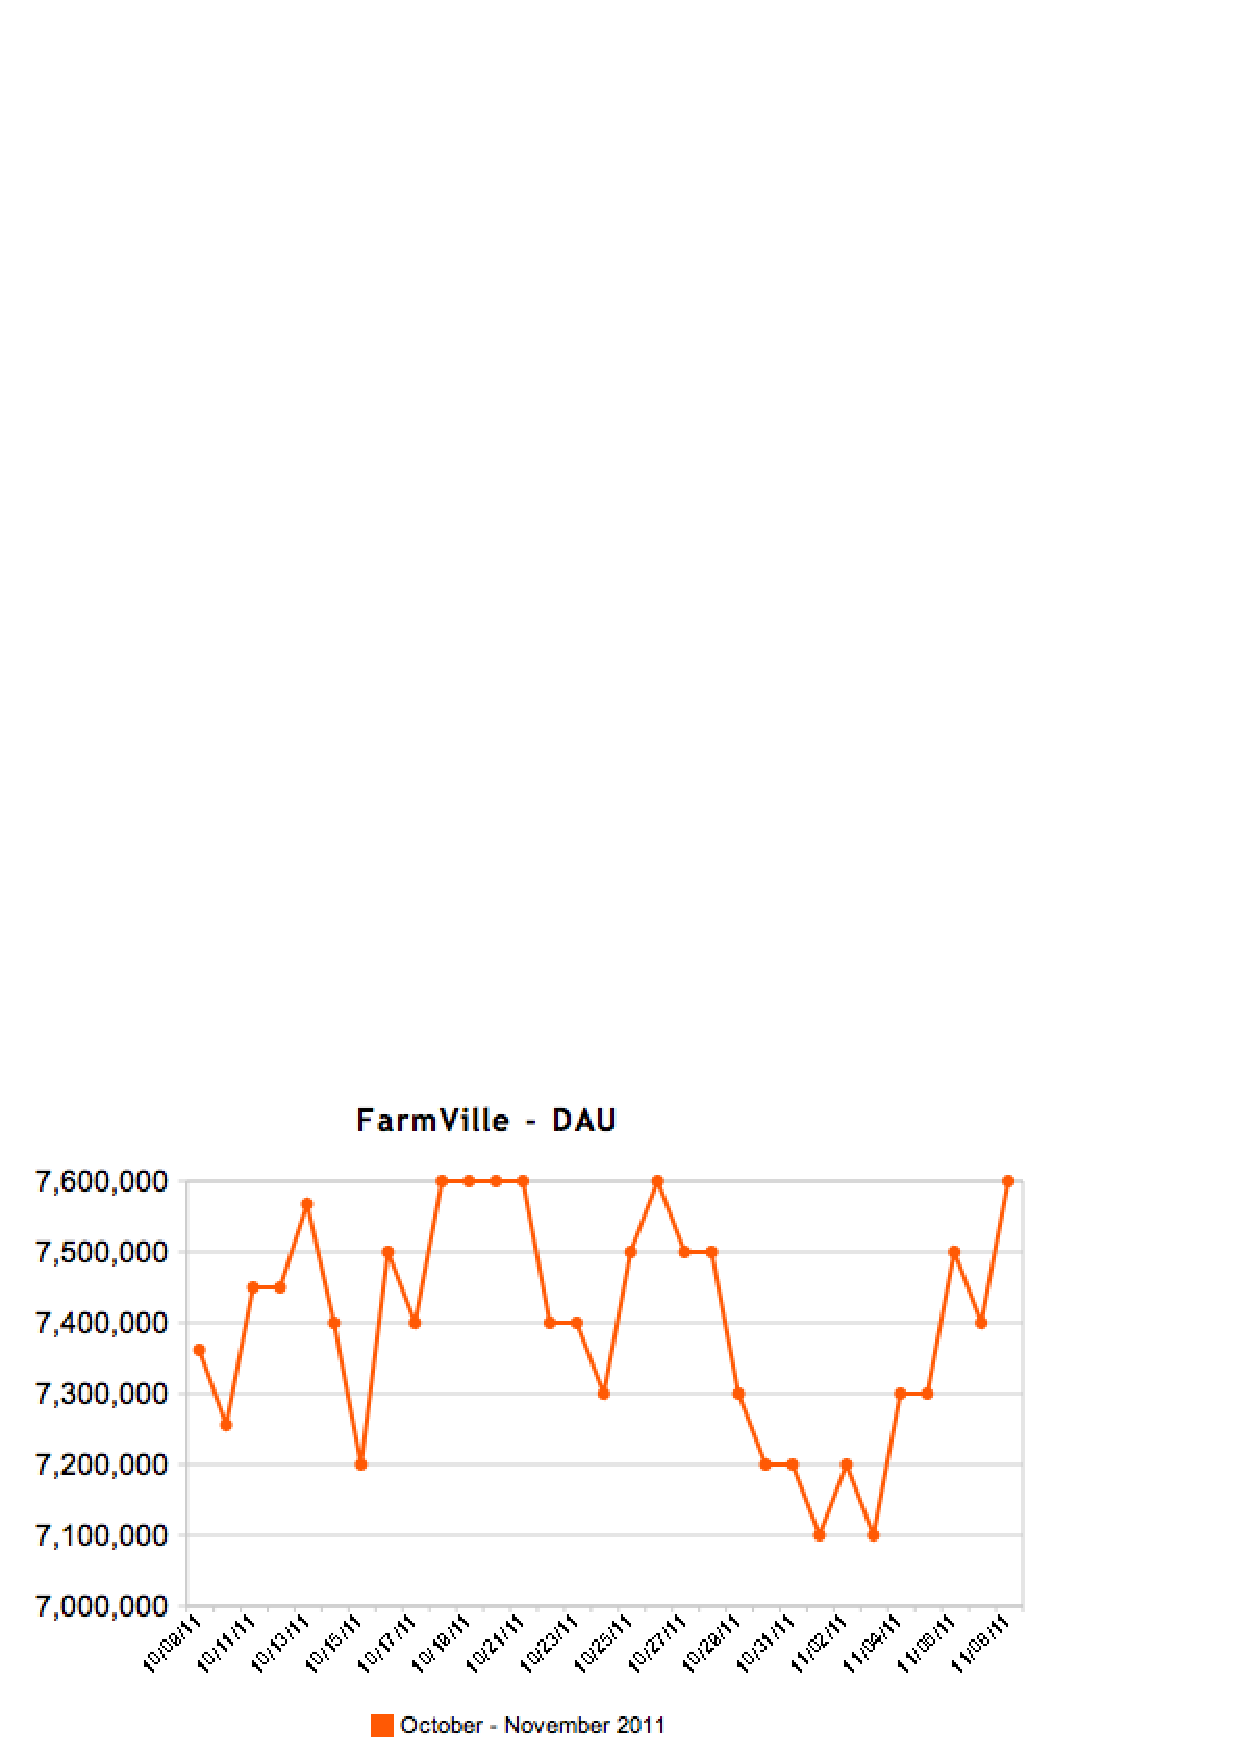
\includegraphics[height=1.85in]{FarmVille2.png}}
		\subfigure[FarmVille MAU]{\label{fig:farmville2}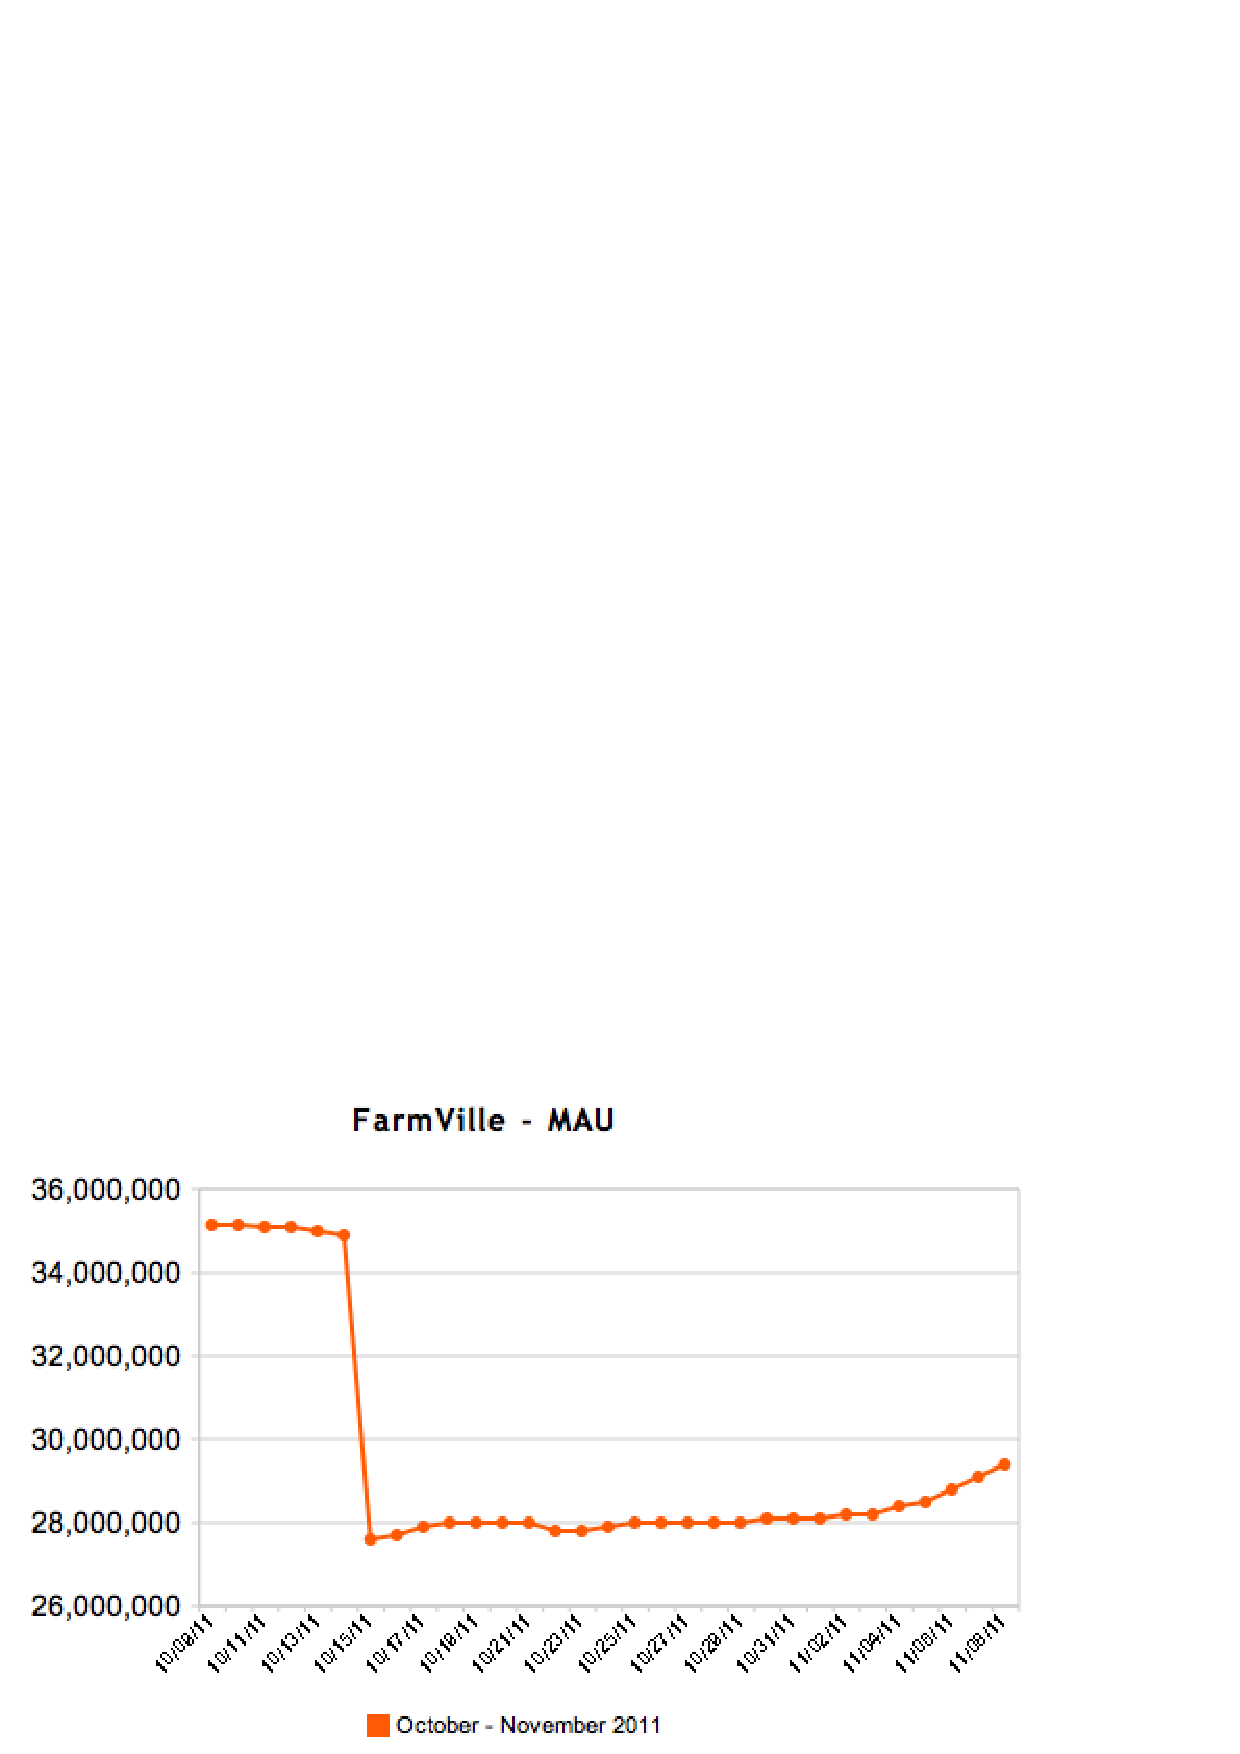
\includegraphics[height=1.85in]{FarmVille1.png}}
		\subfigure[FarmVille DAU/MAU]{\label{fig:farmville3}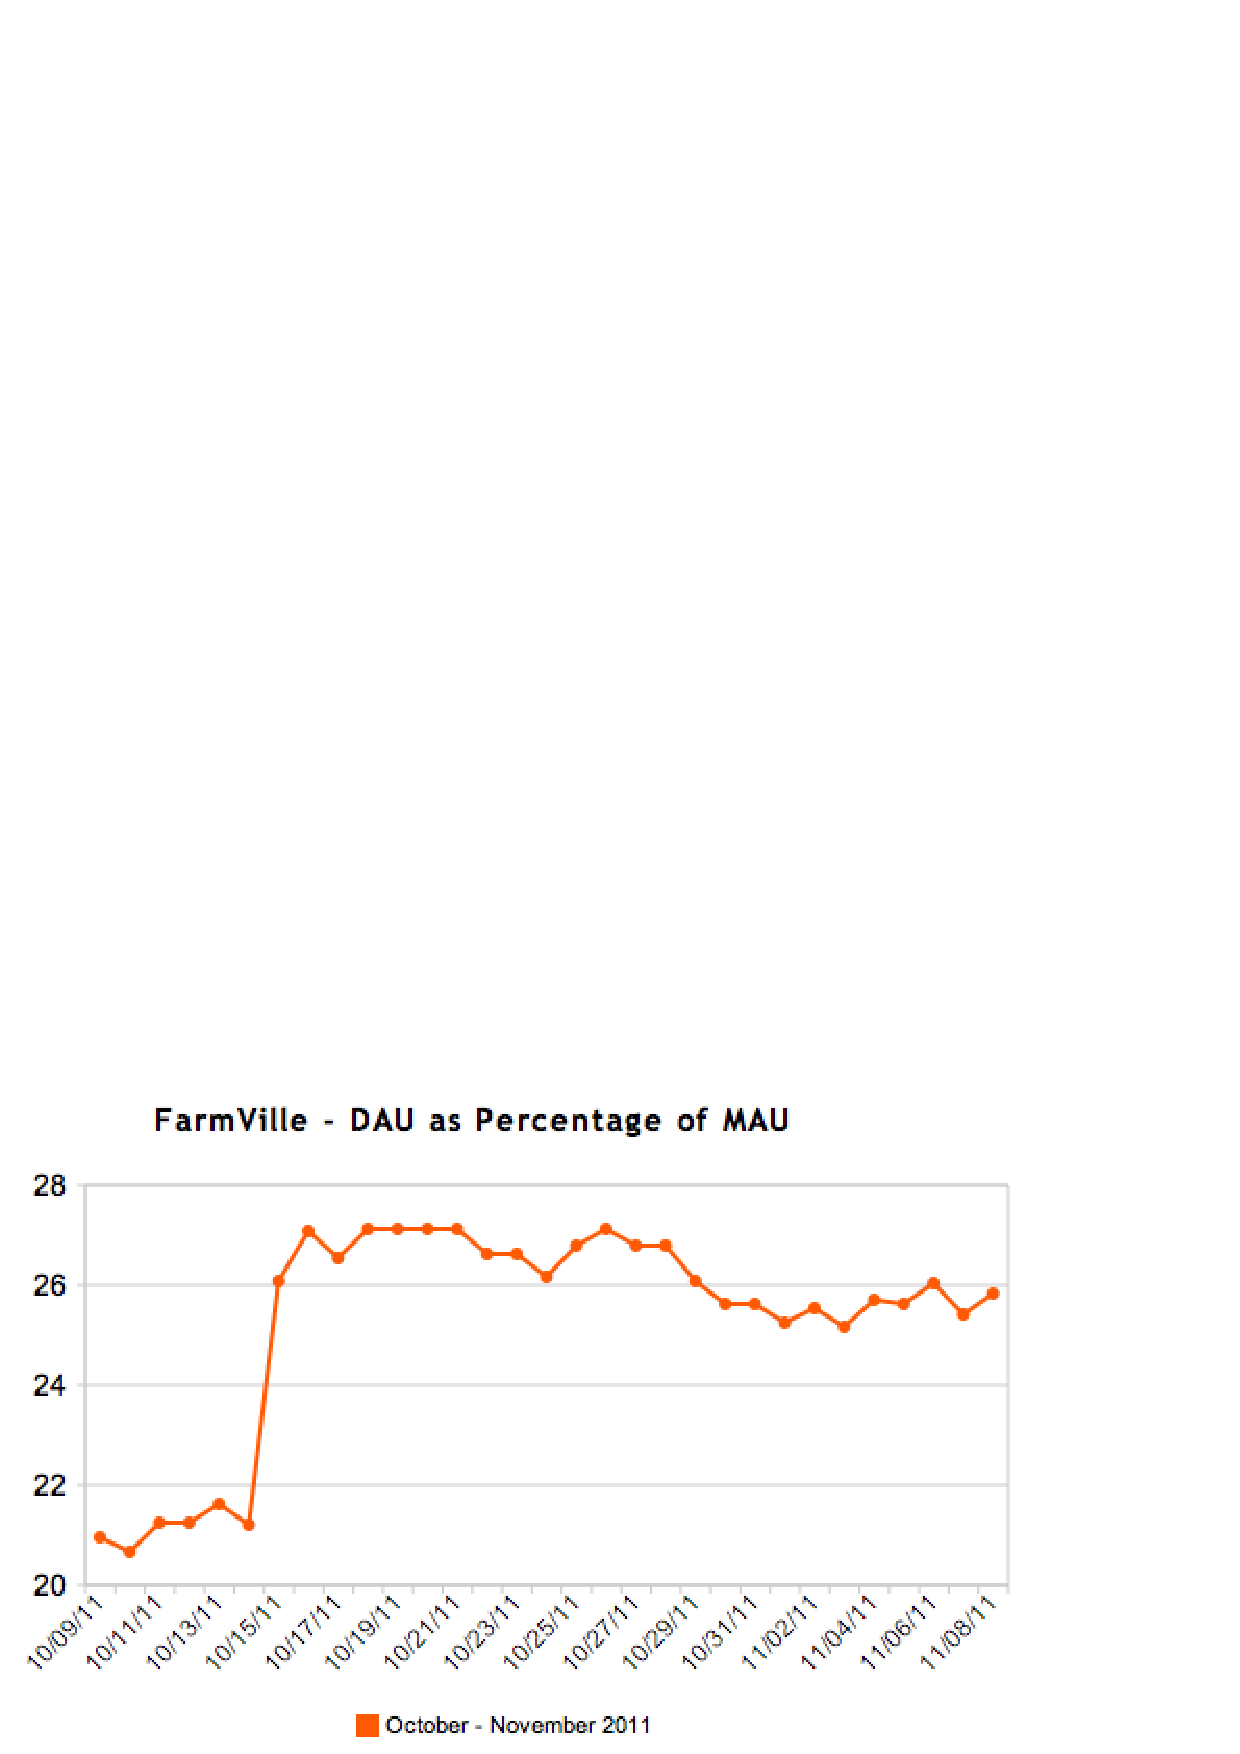
\includegraphics[height=1.85in]{FarmVille3.png}}
		\caption{Social Game Metrics (source: Appdata.com \cite {appdata2011})}
		\label{fig:social-game-metrics}
\end{figure}

Matt Fairchild lists and explains the basic terminology for social games metrics in his blog 
"The Secret Glossary of Social Games Analytics" \cite {Fairchild2010}:

\textbf{ARPU}: Average Revenue Per User (ARPU) is measured as total revenue divided by the number of subscribers. This includes revenue from subscriber fees, virtual goods, affiliate marketing and ad impressions. Because social games are so metrics-heavy, ARPU can be broken down by day, by country, by demographic, or by pretty much any other metric.

\textbf{Churn}: The turnover rate (or �attrition rate�) of a social game�s active players. Churn refers to the constant loss and gain of members, especially high in casual gaming.

\textbf{Cohort}: Cohorts are used for analyzing retention. By organizing users in groups such as ``everyone that visited on June 10th'' and analyzing the percentage that revisit, you can pinpoint what promotions are having the greatest effect.

\textbf{DAU}: Daily Active Users (DAU) is the number of active users over the course of a single day.

\textbf{DAU/MAU}: Comparing Daily Active Users to Monthly Active Users shows roughly how many days per month the average user engages with a game. The DAU/MAU ratio is strongly correlated with social gaming success.

\textbf{Engagement}: Engagement measures how long users spend playing a game. How many features do they access? Are they spending hours or seconds? How many pages does the average user view? What percentage are returning visitors?

\textbf{Entry Event}: An entry event is the first action a user performs when he  enters the game. What do users do first? Which entry events are the most effective at bringing people back? By determining the more popular entry events, you can push more resources towards them, thus increasing retention, engagement and re-engagement.

\textbf{Exit Event}: Exit events are the last actions a user performs before exiting the game. Tracking the Exit Event Distribution helps show why users are disengaging with the game.

\textbf{K Factor}: K Factor measures the virality of a game. K Factor = (Infection Rate) * (Conversion Rate). An Infection Rate is how much a given user exposes the game to other players, such as through status updates or email invites. A conversion rate is when that ``infection'' results in a new sign up. A high K Factor indicates effectiveness of bringing in new players.

\textbf{Lifetime Network Value}: The value a user provides to your network over the course of his entire ``lifetime'' on the network. For instance, is the user contributing to viral effects, evangelizing the game or contributing positively to ARPU? This is compared to the User Acquisition Cost, or how much it costs (via marketing and viral efforts) to bring in new members.

\textbf{MAU}: Like DAU, Monthly Active Users (MAU) tracks the total number of users in a given month.

\textbf{Re-Engagement}: Re-engagement is about how to get users back. It includes re-engaging gamers who have been signed off for an hour, a day, a month, or more. 

\textbf{Retention}: Retention is how well you maintain user base, as the opposite of churn. 
\\\\
Another list of game metrics comes from Kontagent, a user analytics service company. Kontagent summaries the top 10 social game metrics in their 2010 Social Game Summit presentation \cite {Kontagent2010}:

1. Entry Event Distribution

2. Outbound Messages/User

3. Viral Message CTR/Conversion

4. Virality (K-factor) 

5. Engagement

6. Exit Event Distribution

7. Retention - Revisit Rate

8. Lifetime Network Value

9. Conversion to paying users

10. Average Revenue Per Paying User
